\documentclass[11pt]{article}

\usepackage{comment} % enables the use of multi-line comments (\ifx \fi) 
\usepackage[a4paper,margin=1cm]{geometry}
\usepackage[utf8]{inputenc}
\usepackage[ngerman]{isodate}
\usepackage{gensymb}
\usepackage{graphicx}
\usepackage{booktabs}% http://ctan.org/pkg/booktabs
\usepackage{tabularx}
\usepackage{ltablex} % Longtables with tabularx
\usepackage[x11names]{xcolor}
\usepackage{amsmath}
\usepackage{amssymb}
\usepackage{amsthm}
\usepackage{array}
\usepackage{wrapfig}
\usepackage{subcaption}
\usepackage{csquotes}
\usepackage{lscape}
\usepackage{geometry}
\usepackage{multicol}
\usepackage{bm}
\usepackage{enumitem}
\usepackage{hyperref}
\usepackage{mdframed}
\usepackage{scalerel}
\usepackage{stackengine}
\usepackage{mathtools}
\usepackage{pdfpages}

% Bibliography & citing
\usepackage[
	backend=biber,
	style=apa,
	bibstyle=apa,
	citestyle=apa,
	sortlocale=en_UK
]{biblatex}
\addbibresource{Bibliography.bib}
% print the whole bibliography
\nocite{*}

% Code highlighting
\usepackage{minted}
\surroundwithmdframed{minted}

% Be able to caption equations and float them in place
\usepackage{float}

\newmdtheoremenv{theorem}{Theorem}
\geometry{a4paper, margin=2.4cm}
\newtheorem*{remark}{Remark}

\newcommand\equalhat{\mathrel{\stackon[1.5pt]{=}{\stretchto{\scalerel*[\widthof{=}]{\wedge}{\rule{1ex}{3ex}}}{0.5ex}}}}
\newcommand\defeq{\mathrel{\overset{\makebox[0pt]{\mbox{\normalfont\tiny def}}}{=}}}
\newcolumntype{C}{>{\centering\arraybackslash}X}

\DeclarePairedDelimiter\abs{\lvert}{\rvert}
\DeclarePairedDelimiter\norm{\lVert}{\rVert}

\setcounter{tocdepth}{3}
\setcounter{secnumdepth}{3}

\graphicspath{{./img/}}

\begin{document}
	
\title{Analysis of Text Data FS20}
\author{Pascal Baumann\\pascal.baumann@stud.hslu.ch}
\maketitle



For errors or improvement raise an issue or make a pull request on the \href{https://github.com/KilnOfTheSecondFlame/mse_summaries}{github repository}.

\tableofcontents
\newpage

\section{Introduction}
Text analysis consist of a series of operations completed by one or more pieces of software on a sample of written human language, with the goal of extracting useful information.

Applications of text analysis include:
\begin{itemize}[noitemsep]
	\item Analysis
	\begin{itemize}
		\item spell checkers
		\item keyword extraction
		\item authorship attribution
		\item document retrieval
		\item text classification
		\item text mining
		\item sentiment analysis
		\item content-based recommendation
	\end{itemize}
	\item Text Analysis and Generation
	\begin{itemize}
		\item machine translation
		\item automatic question answering
		\item automatic summarisation
	\end{itemize}
	\item Text Generation
	\begin{itemize}
		\item database report generation
		\item weather forecast generation
	\end{itemize}
	\item Analysis, Generation and Interaction
	\begin{itemize}
		\item dialogue systems
		\item assistive technology for teaching or writing
	\end{itemize}
\end{itemize}

Analysis of Text Data lies at the intersection of Machine Learning, Computational Linguistics and Human-Computer Interaction. Artificial Intelligence is applied to human language, while human speech data is a related problem which makes use of different technologies, like signal processing.

\subsection{Basic Concepts in NLP}
Machine Learning is a powerful tool in NLP, thus the same vocabulary is used. For Text Analysis supervised learning is used mostly, where the labelled data is classified by human experts and is called the reference or ground truth.

Significance addresses the key question if the difference between the two systems is really due to the fact that one is better than the other or if it can be explained by randomness. This is easier to compute when cross-validation is used, and paired $t$-tests can be used to compare two systems. Performance scores vary depending on the data set it is difficult to predict actual performance on a data set of a different
nature than the test set, this is called the problem of portability.

\subsection{Key Jargon from Linguistic}
\begin{itemize}
	\item letter
	\item syllable
	\item morpheme: a meaningful morphological unit of a language that cannot be further divided
	\item word
	\item phrase: a group of words standing together as a conceptual unit
	\item clause: a group of words in a sentence that contains a subject and a subject
	\item sentence:
	\begin{itemize}
		\item simple sentence: one independent clause
		\item compound sentence: at least two independent clauses
		\item complex sentence: at least one independent clause and one or more dependent clauses
	\end{itemize}
	\item text
	\item corpus: collection of text, pl. corpora
	\item utterance: an uninterrupted chain of spoken or written language
	\item lexeme: basic abstract unit of meaning that roughly corresponds to a set of forms taken by a single root word - for example run, runs, ran and running are forms of the same lexeme
	\item lemma:  one form chosen by convention as the canonical form of a lexeme - go, goes, went, gone, going for the lexeme \emph{go}
\end{itemize}

\subsection{Utterance Decoding}
Decode its propositional content or logical form first and then combine them. Draw inference to solve ambiguities, guess what is left unsaid and, in general, maximise the likelihood given the context.

\subsection{Lexical Analysis}
The goal of lexical analysis is to understand word forms.
\begin{enumerate}
	\item tokenisation: breaking a text into word tokens
	\item lemmatisation: finding the base form of each word token or lemma
	\item Part of Speech tagging: finding the part of speech each word token corresponds to
	\item Named Entity Recognition:  identification of proper nouns of people, places, organizations
\end{enumerate}

\subsection{Syntactic Analysis}
\begin{itemize}
	\item sentence segmentation or splitting
	\item identifying phrases or chunking
	\item figuring out logical functions
	\item building parse trees or parsing
\end{itemize}

\subsubsection{Constituency Parsing}
With syntactic parsing the connection between words can be understood. Constituency parsing breaks a sentence into its basic building blocks.

\begin{center}
	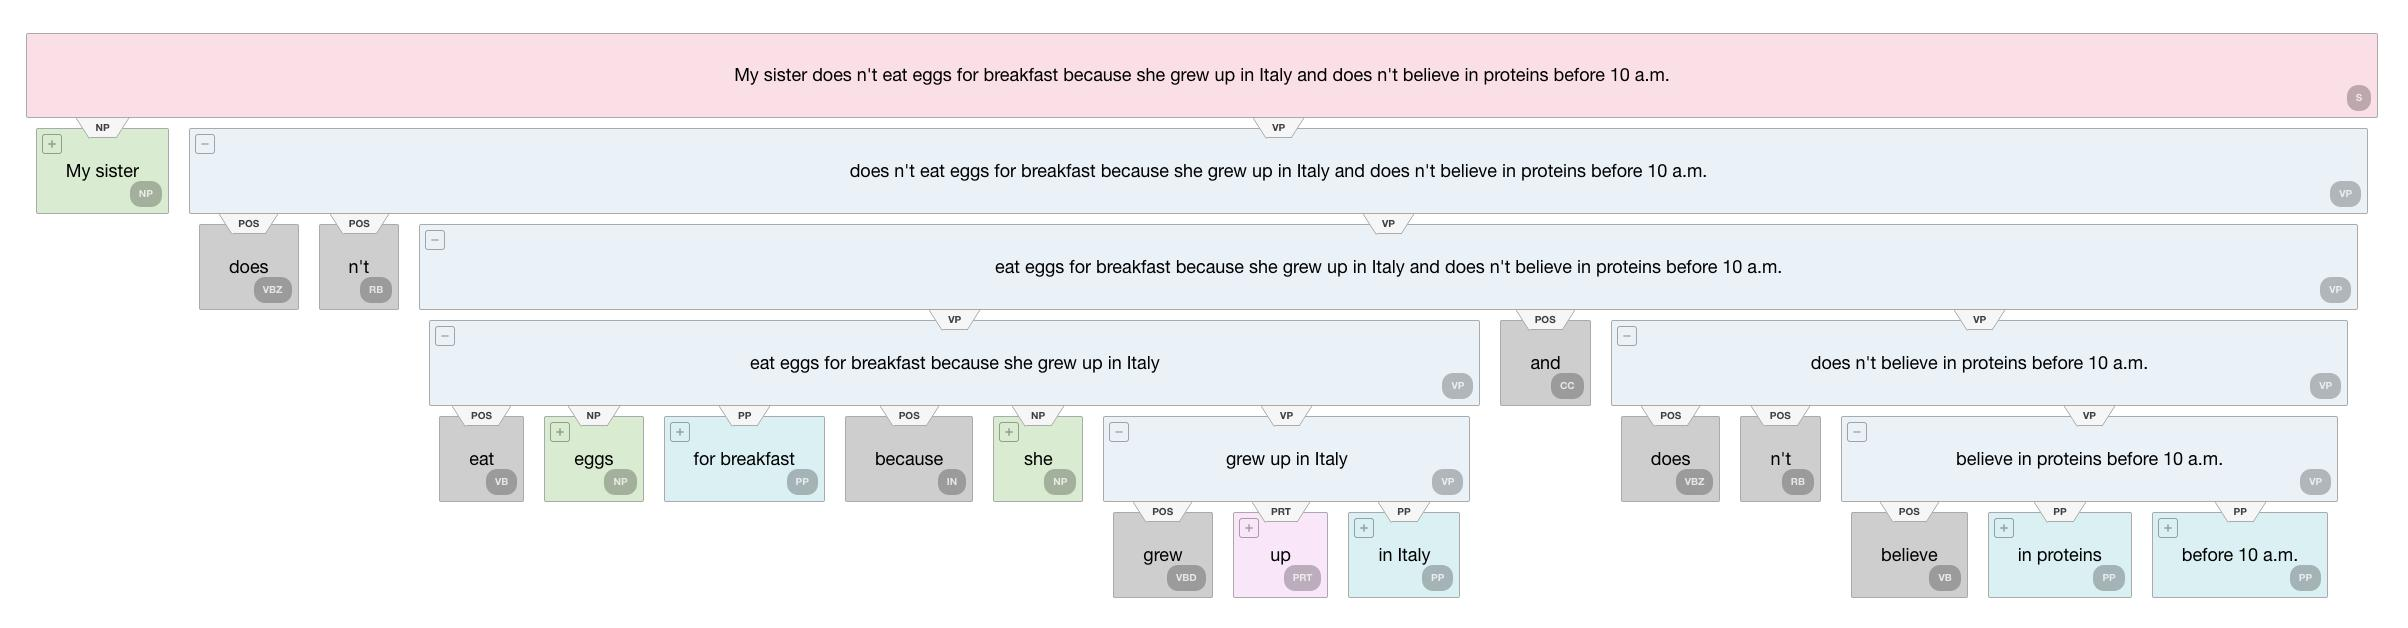
\includegraphics[width=\linewidth]{img/parse_tree_syntactic_parsing}
\end{center}

\subsubsection{Dependency Parsing}
Dependency Parsing helps in understanding what depends on what. The assumption is that the sentence is centred around the verb and what comes first in a sentence is more important than any information that comes after. So anything of the sentence depends on that word or some lower-level information.

\begin{center}
	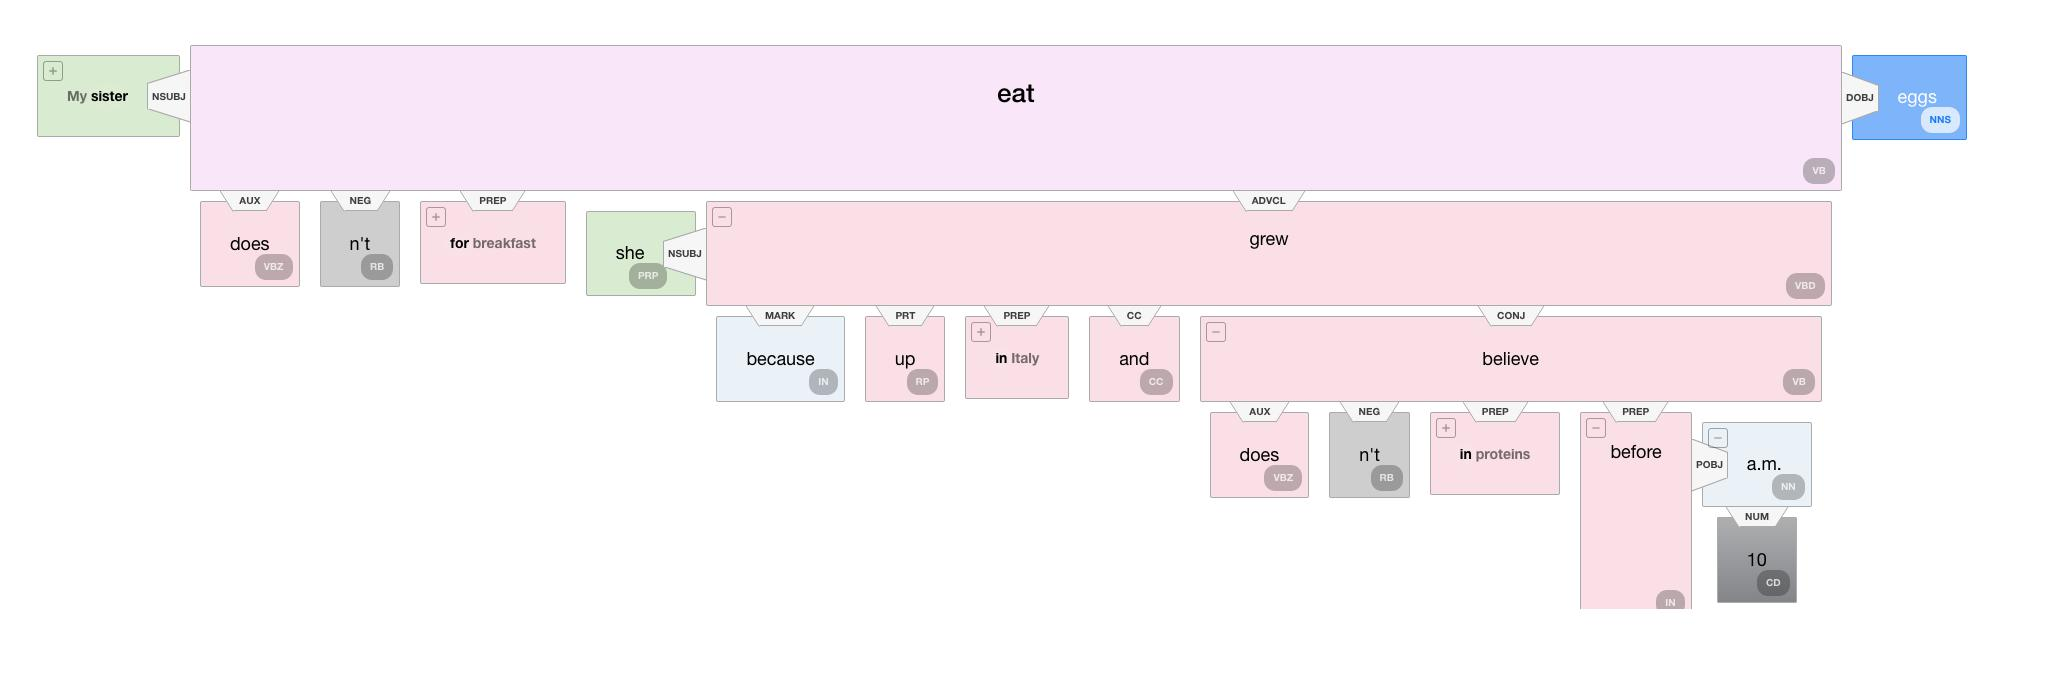
\includegraphics[width=\linewidth]{img/parse_tree_dependency_parsing}
\end{center}

\subsection{Understanding Meaning}
\subsubsection{Semantic Analysis}
\begin{itemize}
	\item word-level
	\begin{itemize}
		\item word sense disambiguation
		\item co-occurrence analysis
	\end{itemize}
	\item sentence-level or text-level
	\begin{itemize}
		\item semantic role labelling
		\item co-reference resolution
	\end{itemize}
\end{itemize}

\subsubsection{Discourse Analysis}
\begin{itemize}
	\item topics
	\item sentiments
	\item speech or dialogue acts
	\item argumentative structures
\end{itemize}

\subsection{Data for Text Analysis}
Text analysis using machine learning requires large amounts of training data and finding suitable data is often a bottleneck due to expense or limited rights. An annotated corpus typically contains a selection of texts based on explicit criteria, metadata like author, date, source, title, sectioning, and annotations in a more or less standardises format.

\subsection{Preprocessing}
Most text processing tasks begin with a set of standard preprocessing steps
\begin{itemize}
	\item Tokenisation: segmentation into tokens
	\item Token normalisation
	\item Segmentation into sentences
	\begin{center}
		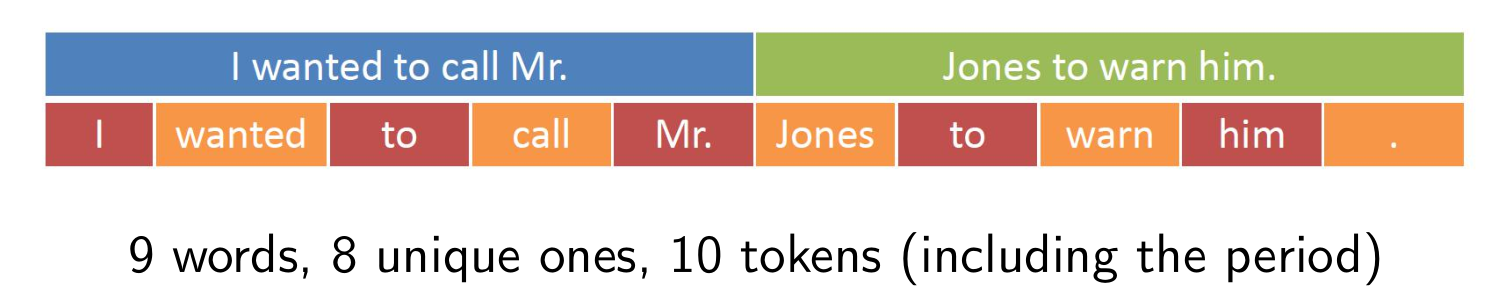
\includegraphics[width=0.8\linewidth]{img/sentence_segmentation}
	\end{center}
	\item There are about 170'000 unique words in the English language at the moment
\end{itemize}

\subsubsection{Tokens and Types}
Tokens are the words on the page, while the type is the word forms. Counting the types requires lemmatisation, which is finding the lemma or base form for each word.

\subsubsection{Tokenisation and Normalisation}
Not as straightforward as one may think
\begin{itemize}
	\item punctuation
	\begin{itemize}
		\item periods and commas appear within words or abbreviations
		\item special tokens in mail addresses or tweets
		\item apostrophes
	\end{itemize}
	\item capital letters
	\item compound words
	\begin{itemize}
		\item problem complicated without dashes
		\item German words
		\item proper names
	\end{itemize}
\end{itemize}

\subsubsection{Sentence Segmentation}
Can be easier or more difficult depending on the source text formatting. If no particular information is available from the layout, punctuations and casing can be used. While question and exclamation marks are quite reliable indicator of sentences periods are not. A good approach is to try to combine Tokenisation and Sentence Splitting, focusing on full stops.

\section{Text Classification}
The goal of text classification is to assign text documents to one or more categories. There is a predefined set of classes, in which previously unseen documents are assigned to. If there are only two classes this is a binary classification problem.

To tackle this problem there are different strategies: (a) have hard-coded rules carefully crafted by an expert on the basis on combinations of words or other features, (b) through supervised machine learning with understanding building on semantic representation of texts and labels or (c) supervised machine learning without understanding where word-based features are derived from text and the relationship between features and labels from the training texts.

Stopwords are words like conjunctions or preposition, which may not have meaning given the task at hand.

\subsection{Formalising Text Classification}

\begin{itemize}[label=]
	\item Input
	\begin{itemize}
		\item a set of documents $D$
		\item a fixed set $N$ of classes $C$
		\item a training set of $M$ hand-labelled documents $(d_1 C_1),(d_2 C_2), \dots (d_M C_M)$
	\end{itemize}
	\item Output
	\begin{itemize}
		\item a mapping $D\rightarrow C$ that associates a predicted class $c\in C$ to each document $d\in D$
	\end{itemize}
\end{itemize}

\subsection{Naïve Bayes Classifier}
For a document $d$ and a class $c$

\begin{equation*}
	P(c|d) = \frac{P(d|c)P(c)}{P(d)}
\end{equation*}

\noindent
Maximum A Posteriori (MAP) classifier:
\begin{equation*}
	c_{\text{MAP}} = \underset{c\in C}{\text{argmax}} \frac{P(d|c) P(c)}{P(d)} = \underset{c\in C}{\text{argmax}} P(d|c) P(c)
\end{equation*}

Dropping the denominator does not change $c_{\text{MAP}}$ because $P(d)$ has no effect on argmax. In practice, the evidence a machine can observe is not the human-readable document $d$, but a number of features $x_1,\dots,x_N$ obtained based on $d$ and a MAP-classifier
\begin{equation*}
	c_MAP = \underset{c\in C}{\text{argmax}} P(x_1, x_2, \dots , x_N | c) P(c)
\end{equation*}

\noindent
Given a vocabulary of V words a feature can be if a word appears in a document $d$ or how often it appears
\begin{itemize}
	\item \textbf{Bernoulli Model} represent $d$ as $(e_1, \dots, e_V)$ where $e_i =1$ if the word $i$ is in $d$ and $e_i = 0$ otherwise
	\item \textbf{Multinomial Model} represent $d$ as $f_1, \dots, f_V)$ where $f_i$ is the number of occurrences of word $i$ in $d$
\end{itemize}

The Naïve Bayes independence assumption is that given a class $c$ the \textbf{features are independent}
\begin{equation*}
	P(x_1, x_2, \dots , x_N | c) = P(x_1|c)\cdot P(x_2|c) \cdots P(x_N|c) = \prod_{k=1}^{n}P(x_k|c)
\end{equation*}

$P(c)$ and $P(x_k|c)$ need to be computed, $P(c)$ can be estimated based on the frequency of each class in the training data, and $P(x_k|c)$ depends on the chosen feature representation.

In the so called Bag-Of-Word Model $x_k$ is the feature representation of the words in the documents. The position of the individual words can usually be ignored.

\subsection{Multinomial Naïve Bayes}
Represent every token in $d$ as a feature vector $x_i = f_i$ , where $f_i$ is the number of occurrences of token $i$ in $d$. Then $P(x_i|c)$ can be estimated as $\frac{\text{number of occurrences of token }i\text{ in }c}{\text{total number of tokens in }c}$. For simplicity $P(w|c)$ can be written to refer to the probability of finding token $w$ in class $c$.

\begin{enumerate}
	\item Normalise the training data (remove stop words, remove punctuation, set all characters to lowercase)
	\item Assemble vocabulary (list of unique meaningful words)
	\item Count the number of occurrences of each word in each class and divide by the total number of words in each class
\end{enumerate}

\subsection{Practical Complications}
If a word $w$ from the vocabulary (which contains $V$ tokens) is never in class $c$ in the training data, we will estimate $P(w|c) = 0$, which causes $c_{\text{corpus}}=\underset{c\in C}{\text{argmax}}P(c)\prod_{k=1}^{N}P(x_k|c)=0$.

\begin{remark}
	Zero probabilities cannot be conditioned away, no matter the other evidence!\\ - Dan Jurafsky
\end{remark}

The typical solution to this is to do Laplace Smoothing like this
\begin{equation*}
	P(w|c)\text{ can be estimated as }\frac{\text{number of occurrences of token $w$ in class } c + 1}{\text{total number of tokens in class } c+V}
\end{equation*}
This prevents probabilities of zero to occur.

\subsection{Metrics}
\begin{itemize}[leftmargin=*, labelindent=3cm, labelsep=1cm]
	\item[True Positive] Sample $c$ classified correctly
	\item[False Positive] Non-$c$ sample incorrectly classified as $c$
	\item[True Negative] Non-$c$ sample classified correctly
	\item[False Negative] Sample $c$ classified incorrectly as non-$c$
\end{itemize}

\begingroup
	\renewcommand{\arraystretch}{1.5}
	\begin{tabularx}{\linewidth}{rX}
		Accuracy & $ \frac{\sum TP}{\sum \text{all elements}} $ \\
		Precision & $\frac{TP}{TP + FP}$\\
		Recall & $ \frac{TP}{TP + FN} $\\
	\end{tabularx}
\endgroup

\section{Sentiment Analysis}
Sentiment analysis tries to understand the emotional state of the author of a text, and is also called opinion mining but can be extremely hard. In principle text classification and sentiment analysis are very different, but there are some striking similarities as the text can reflect a positive or a negative emotional state which can be utilised.

\subsection{Framing Sentiment Analysis}
Sentiment analysis is commonly framed as \textbf{attitude detection}
\begin{itemize}
	\item \emph{Attitude} is an enduring disposition toward someone or something with an emotional connotation
	\item The attitude can be broken down in quintuplets
	\begin{enumerate}
		\item opinion holder
		\item target entity
		\item aspect: specific feature of the target that the opinion is about
		\item type: most commonly {\color{green} positive}, {\color{red} negative}, {\color{gray} neutral} and with an indication of strength
		\item time when this opinion was expressed
	\end{enumerate}
	\item knowing the opinion without knowing the opinion target is of limited use
\end{itemize}

\subsection{Tokenisation Challenges}
\begin{itemize}
	\item Isolating emoticons
	\item Respecting domain-specific markup like \mintinline{html}{<strong>really bad idea</strong>}
	\item Capturing masked curses
	\item Selective true-casing
	\item Normalised lengthening, as "YAAAAAAY" is equivalent to "YAY" no matter how it is written
	\item Capturing important multi-word expressions and idioms
\end{itemize}

\subsubsection{Dealing With Negations}
A simple effective workaround by Das and Chen is to prepend \texttt{NOT\_} to every word between a negation and a clause-level punctuation mark.

\subsubsection{More Complications}
\begin{itemize}
	\item Modal adverbs like \emph{quite possibly, totally}
	\item Thwarted expectations "\emph{It was hailed as brilliant, unprecedented artistic achievement worthy of multiple Oscars}"
	\item Non-literal language "\emph{Like 50 hours long}"
\end{itemize}

\subsection{Various Degrees of Complexity}
In principle, all quintuplets in a document should be discovered, which would allow to represent unstructured information in a structured form. However, this is extremely hard to do. In practice, simplified forms of sentiment analysis are typically solved
\begin{itemize}
	\item Document-level sentiment classification
	\item Sentence-level sentiment classification
	\item Aspect-level sentiment classification
\end{itemize}
Though simplified, these forms of sentiment analysis are still hard to do with subtlety and sarcasm complicating the task.

\subsubsection{Document-level Sentiment Classification}
Does the document reflect an overall {\color{green} positive} or {\color{red} negative} view? The approach is the same as for text classification
\begin{enumerate}
	\item tokenisation
	\item feature extraction
	\item classification (Naïve Bayes, MaxEnt, SVM)
	\item Two or Three classes \{ {\color{green} positive} $\vert$ {\color{red} negative} $\vert$ ({\color{gray} neutral}) \}
\end{enumerate}

\subsection{Generative versus Discriminative Models}
In Naïve Bayes, for a document $d$ and each class $c$:
\begin{itemize}
	\item Estimate $P(d|c)$ and $P(c)$ directly from the training data
	\item Learn a model of $P(d\cap c) = P(d|c)\cdot P(c)$
	\item Use Bayes' rule to compute $P(c|d)=\dfrac{P(d|c)\cdot P(c)}{P(d)}$
	\item Pick the class that maximises $P(c|d)$ over all classes
\end{itemize}
This is called a \textbf{generative model}: Which class $c$ is most likely to have generated my test sample $d$, given the $P(d\cap c)$ that was estimated.

\noindent
The alternative is a \textbf{discriminative model} that models $P(c|d)$ directly.

\subsection{Discriminative Model: Maximum Entropy}
Entropy in information theory refers to a measure of the information content, where highly probable events carry very little information and if all events are equally likely there is maximum entropy. A prediction on which one will occur is impossible and when a event occurs there is a lot of learning.
\begin{itemize}
	\item Suppose movie reviews get classified into \{ {\color{Green3} positive} $\vert$ {\color{Firebrick3} negative} $\vert$ ({\color{gray} neutral}) \}
	\item In the training corpus 90\% of the sample containing the word \texttt{love} are tagged as {\color{Green3} positive}
	\item Let it further be that a test sample with the word \texttt{love} is 90\% likely to be positive and equally likely to be either {\color{Firebrick3} negative} (10\%) or {\color{gray} neutral} (10\%)
	\item All other things unknown are assumed to be equally likely (maximum entropy)
\end{itemize}
Unlike in text classification, topic words are not as important as \textbf{sentiment words} that carry an emotional charge, but the mapping between emotional states and the written word can be exceedingly subtle
\begin{itemize}[label=-]
	\item {\color{Green3} good}, {\color{Green3} splendid}, {\color{Green3} nice}
	\item {\color{Firebrick3} bad}, {\color{Firebrick3} racist}, {\color{Firebrick3} dismal}
\end{itemize}

\subsection{Unsupervised Sentiment Classification}
\begin{enumerate}
	\item Use a Part-Of-Speech tagger to identify phrases with adjectives and adverbs
	\item Estimate the semantic orientation
	\item Classify based on the average semantic orientation
\end{enumerate}
Semantic orientation is computed based on Pointwise Mutual Informaiton (PMI)
\begin{equation*}
\text{PMI} (w_1,w_2) = \log_2 \left( \frac{P(w_1,w_2)}{P(w_1)P(w_2)} \right) = \log_2 \left( \frac{P(w_1 | w_2)}{P(w_1)} \right) = \log_2 \left( \frac{P(w_2 | w_1)}{P(w2)} \right)
\end{equation*}
PMI is computed using approximate probabilities with normalised word counts in a corpus. Or the web can be used as a corpus using the number of hits from a search engine when $w_1$ and $w_2$ are searched. Following Barrière (2016) the number of hits of \texttt{the, a, of} are used, which results in a total of $2.527\cdot 10^10$ hits.
\subsubsection{Example PMI of Academy and Awards}
\begin{itemize}
	\item $w_1 = \text{\texttt{Academy}}$, $w_2 = \text{\texttt{Awards}}$
	\item $P(w_1,w_2) \propto \text{\#\texttt{Academy} AND \texttt{Awards}} \approx 1.01\cdot 10^9\text{hits}$
	\item $P(w_1) \propto \text{\#\texttt{Academy}} \approx 1.94\cdot 10^9 \text{hits}$
	\item $P(w_2) \propto\text{\#\texttt{Awards}} \approx 5.57\cdot 10^9\text{hits} $
	\item $\text{PMI}(w_1,w_2) \approx \log_2\left( \frac{1.01\cdot 10^9\cdot2.527\cdot 10^10}{1.94\cdot 10^9\cdot 5.57\cdot 10^9} \right)\approx 1.24 $
\end{itemize}
Two words with high PMI are very likely to occur jointly, while two words with low PMI are very likely to occur separately. PMI can also be used to compute Semantic Orientation (SO), by computing the PMI of selected bigrams with reference words.

\section{Representation and Querying}
User has information needs and expresses them as a text query, the system matches the query with the documents and returns results. The system is using system-specific document or query representations to make comparison possible. The problem is, that computers have difficulties to work with text directly, so the text has to be transformed into something the machine can work with, usually a vector of numbers.

\subsection{Document Representation}
The idea is to count the words that are shared between documents. The higher the score, the more words are shared, the higher the apparent similarity between documents. But lexemes and capitalisation makes this task harder.
\begin{figure}[H]
	\centering
	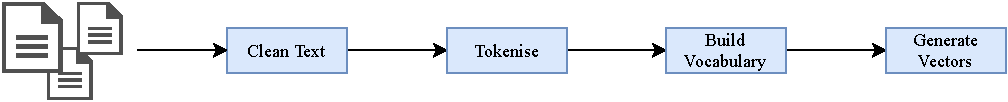
\includegraphics[width=0.8\linewidth]{img/preprocessing_pipeline}
	\caption{Preprocessing pipeline for text}
	\label{fig:preprocessingpipeline}
\end{figure}
The actual steps taken in the preprocessing depends heavily on the use case.

\subsubsection{Clean Text}
\begin{itemize}[noitemsep]
	\item Remove markup
	\item Expand contractions
	\item Truecase
	\item Remove stopwords
	\item Only keep specific word forms
\end{itemize}

\subsubsection{Tokenise}
\begin{itemize}[noitemsep]
	\item Tokenise
	\item Lemmatisation
	\item Stemming\\
	Reduces inflected words to their stem, the root or base forms, even if the stem itself is not a valid word in the language
\end{itemize}

\subsection{Scoring with Jaccard Similarity}
The idea to count the words that are shared between documents to account for similarity stays the same. But the Jaccard Similarity is defined as the size of intersection divided by the size of the union of two sets.

\noindent
\begin{minipage}{0.6\linewidth}
	\begin{equation*}
	J(\text{document}_1,\text{document}_2) = \frac{\text{document}_1\cap\text{document}_2}{\text{document}_1\cup\text{document}_2}
	\end{equation*}
\end{minipage}
\begin{minipage}{0.4\linewidth}
	\begin{center}
		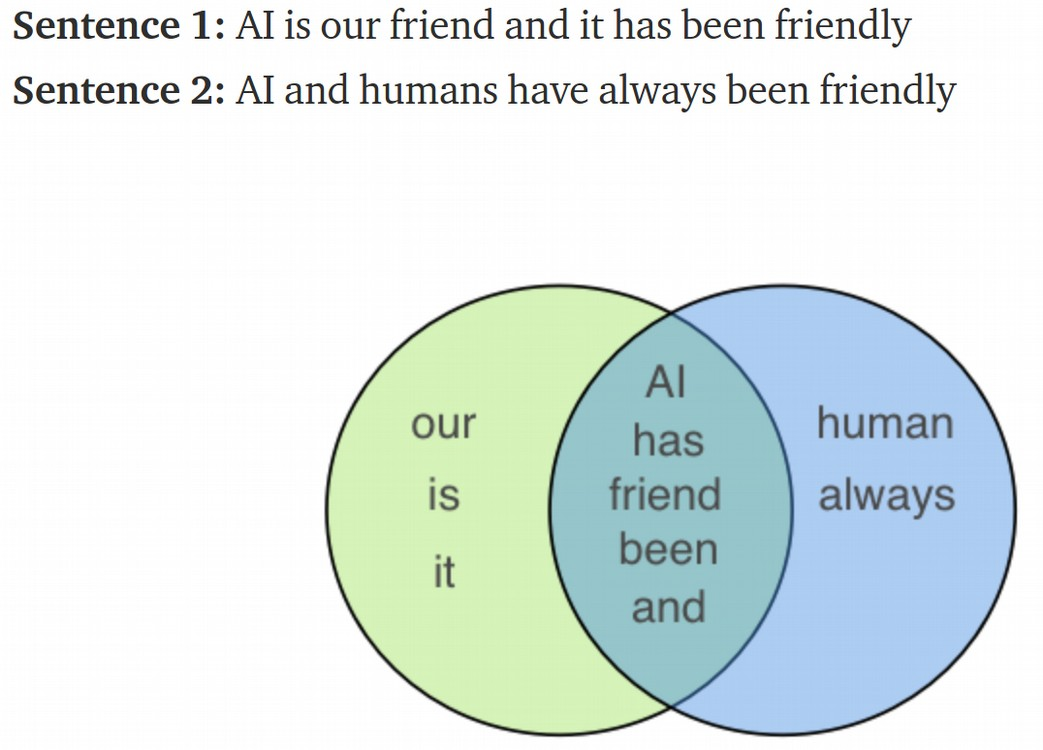
\includegraphics[width=0.9\linewidth]{img/jaccard_set}
	\end{center}
\end{minipage}
Jaccard similarity has the issue of preferring short documents and that it ignores the number a word is occurring.

\subsection{Bag of Words Model}
Focuses on the number of occurrence of words, with the intuition that if a queried word occurs more in the document it is more relevant.
\begin{center}
	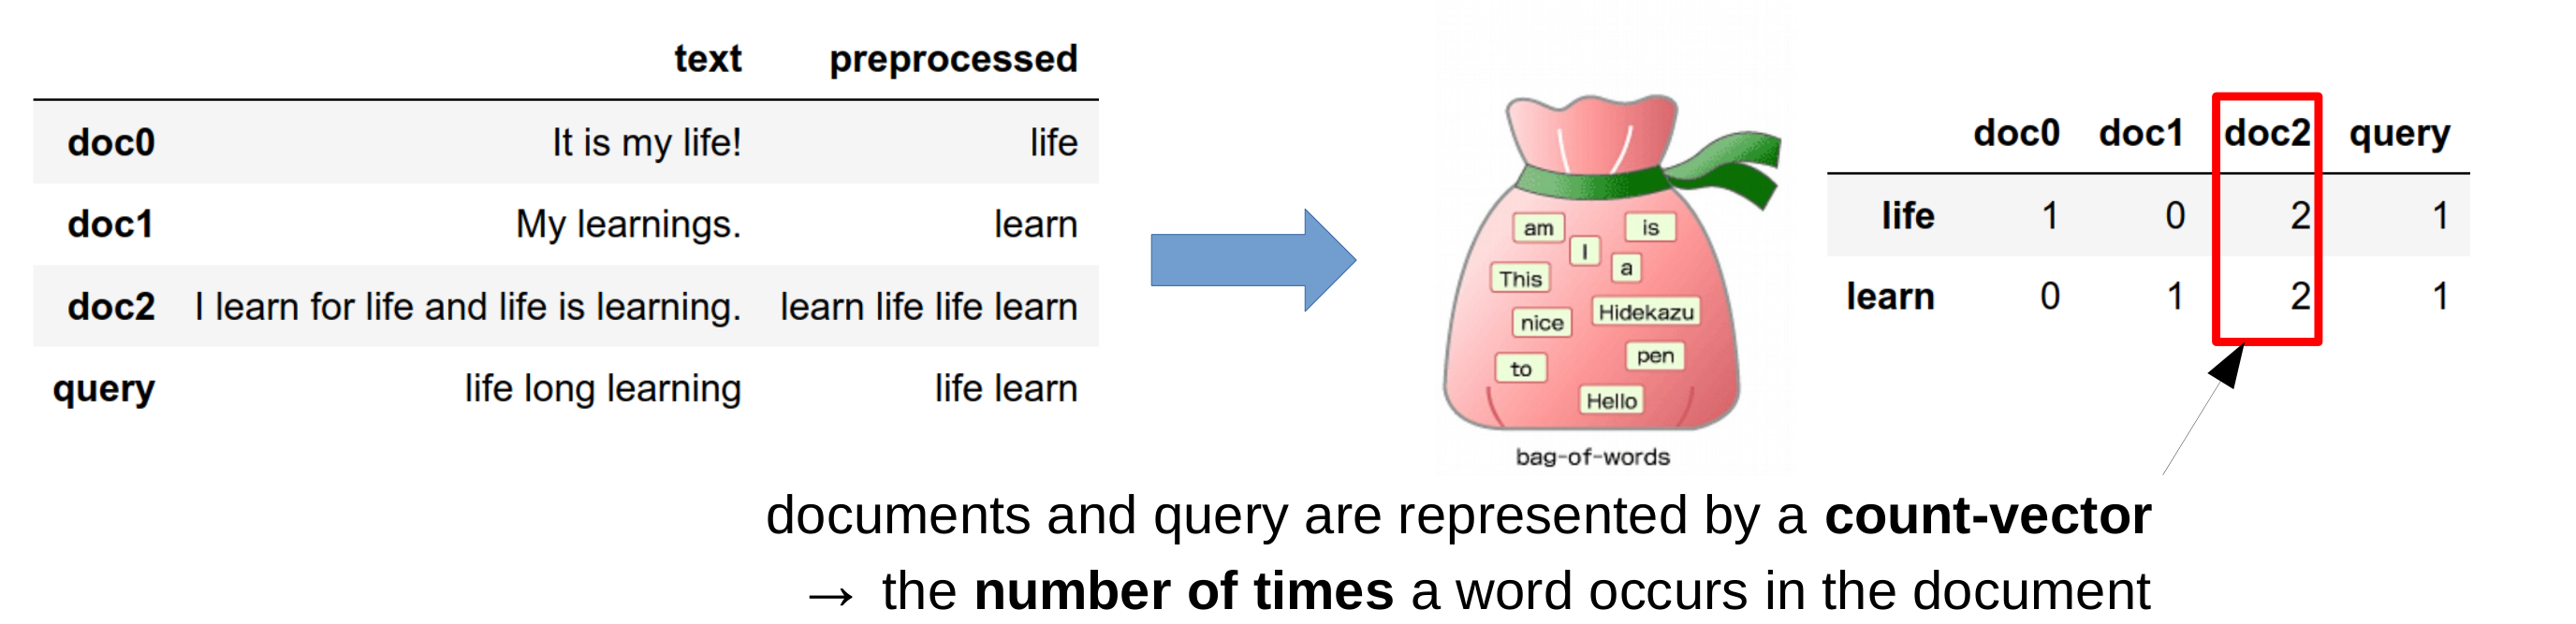
\includegraphics[width=0.8\linewidth]{img/bagofwords_model}
\end{center}
However the Bag of Words model does not consider the ordering of words in a document, and the words must precisely match.

\subsection{Term Frequency Weighting and Transformation}
The raw term frequency is not necessarily the most desirable attribute. A document where a query word occurs more should be handled as more relevant, but a document with 50 occurrences should not be treated 50 times more important than a document with only five occurrences. Thus the relevance should increase sublinear with term frequency
\begin{equation*}
	\text{TF}_{\text{document}} = \underset{\text{word}\in\text{query}\cap\text{document}}{\sum}\log\left( 1 + \text{count}(\text{word},\text{document}) \right)
\end{equation*}
\begin{figure}[H]
	\centering
	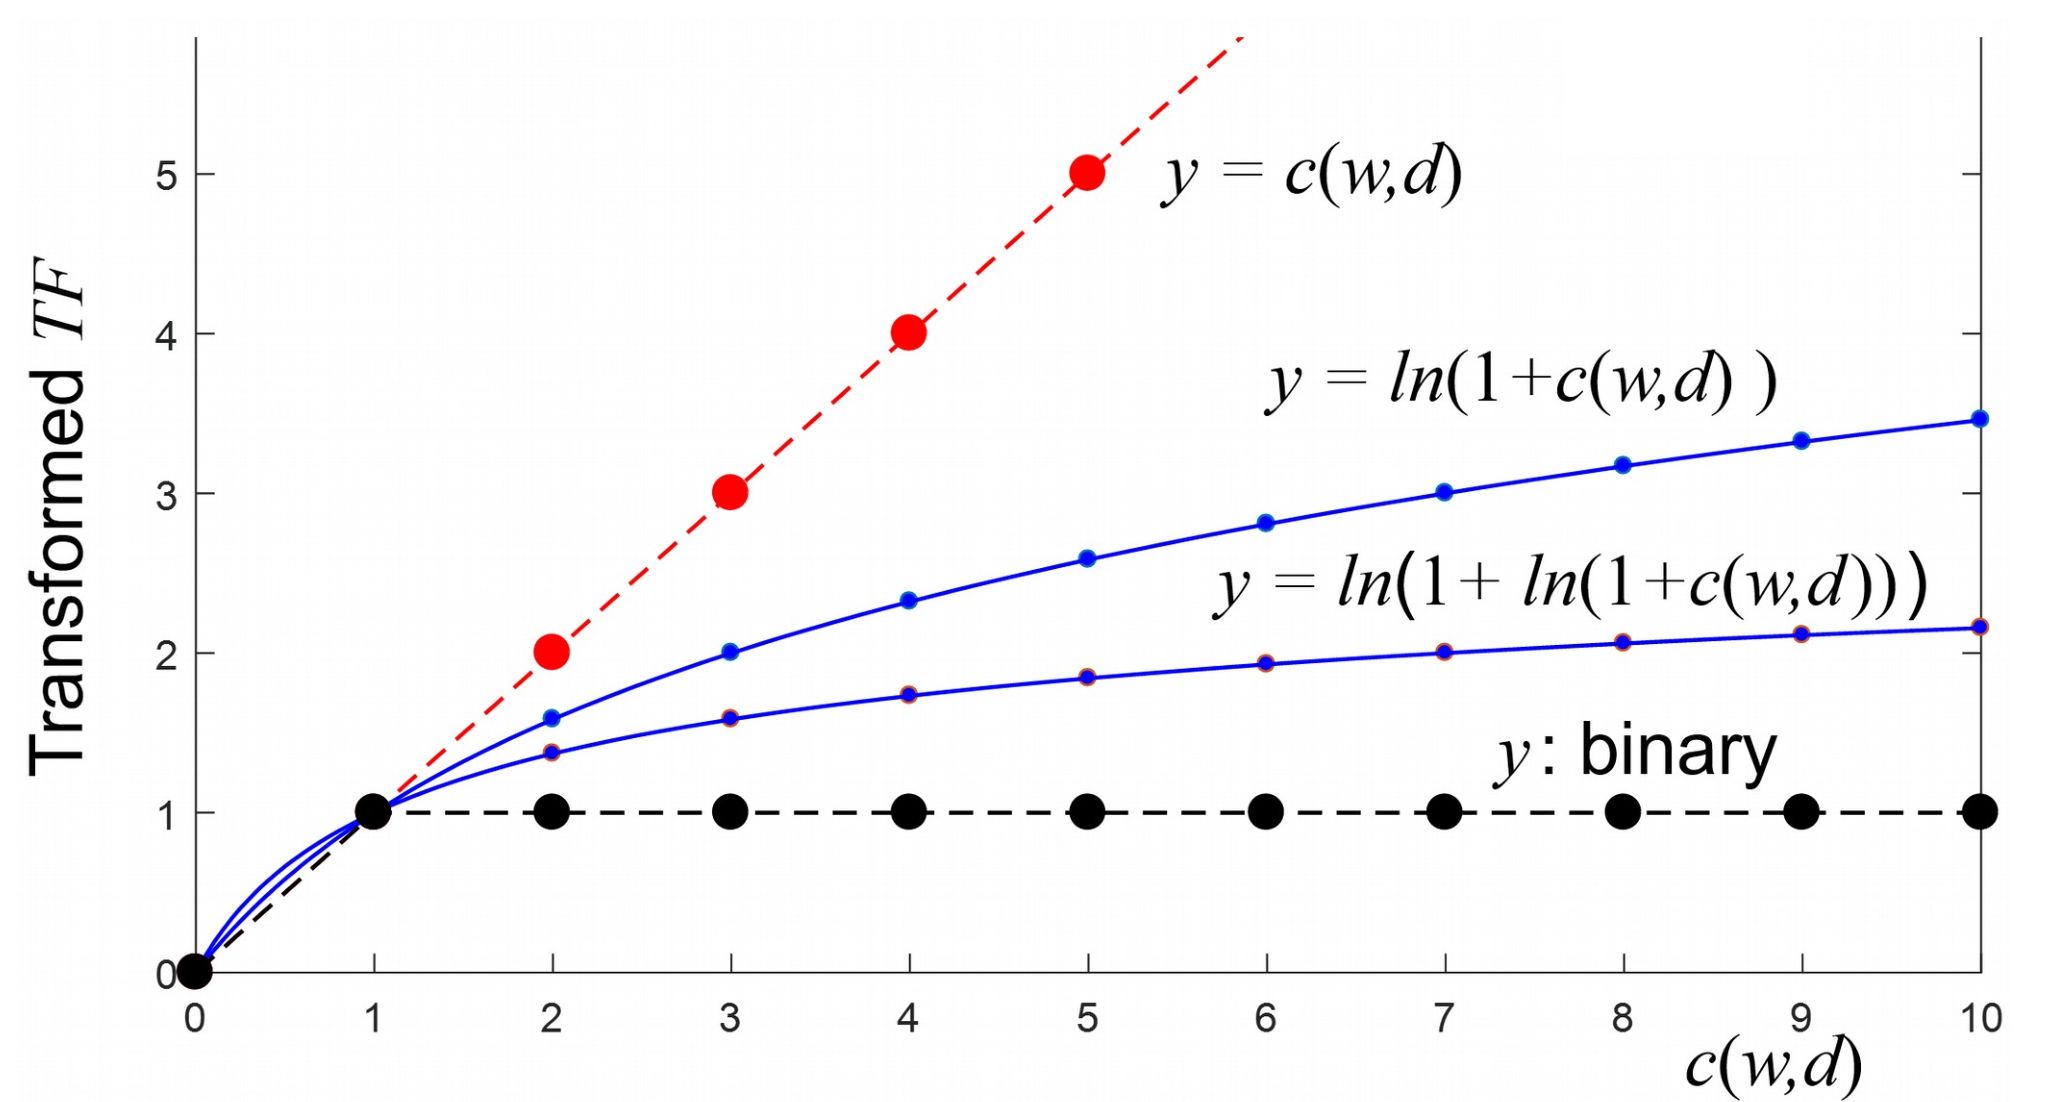
\includegraphics[width=0.6\linewidth]{img/term_frequency_transformation}
	\caption{A sublinear transformation avoids the dominance of single words}
	\label{fig:termfrequencytransformation}
\end{figure}

\subsubsection{(Best Matching) BM25 Term Frequency Transformation}
\begin{equation*}
	y = \frac{(k+1)\cdot c(w,d)}{k+c(w,d)}
\end{equation*}

\subsection{Inverse Document Frequency}
The problem with term frequency lies in the fact that highly frequent words dominate the analysis, but rare and domain specific words may be more informative semantically. Thus positive weights for frequent words but lower weights than for rare words are desirable.
\begin{itemize}[label=]
	\item $\text{DF}_w$: Document Frequency, the number of documents containing word $w$, is the inverse measure of the informativeness of word $w$
	\item $N$: total number of documents in the collection
\end{itemize}
\begin{equation*}
	\text{IDF}_{word}=\log\left(\frac{N}{\text{DF}_{word}}\right)
\end{equation*}
The logarithm is used to dampen the effect of IDF.
\begin{figure}[H]
	\centering
	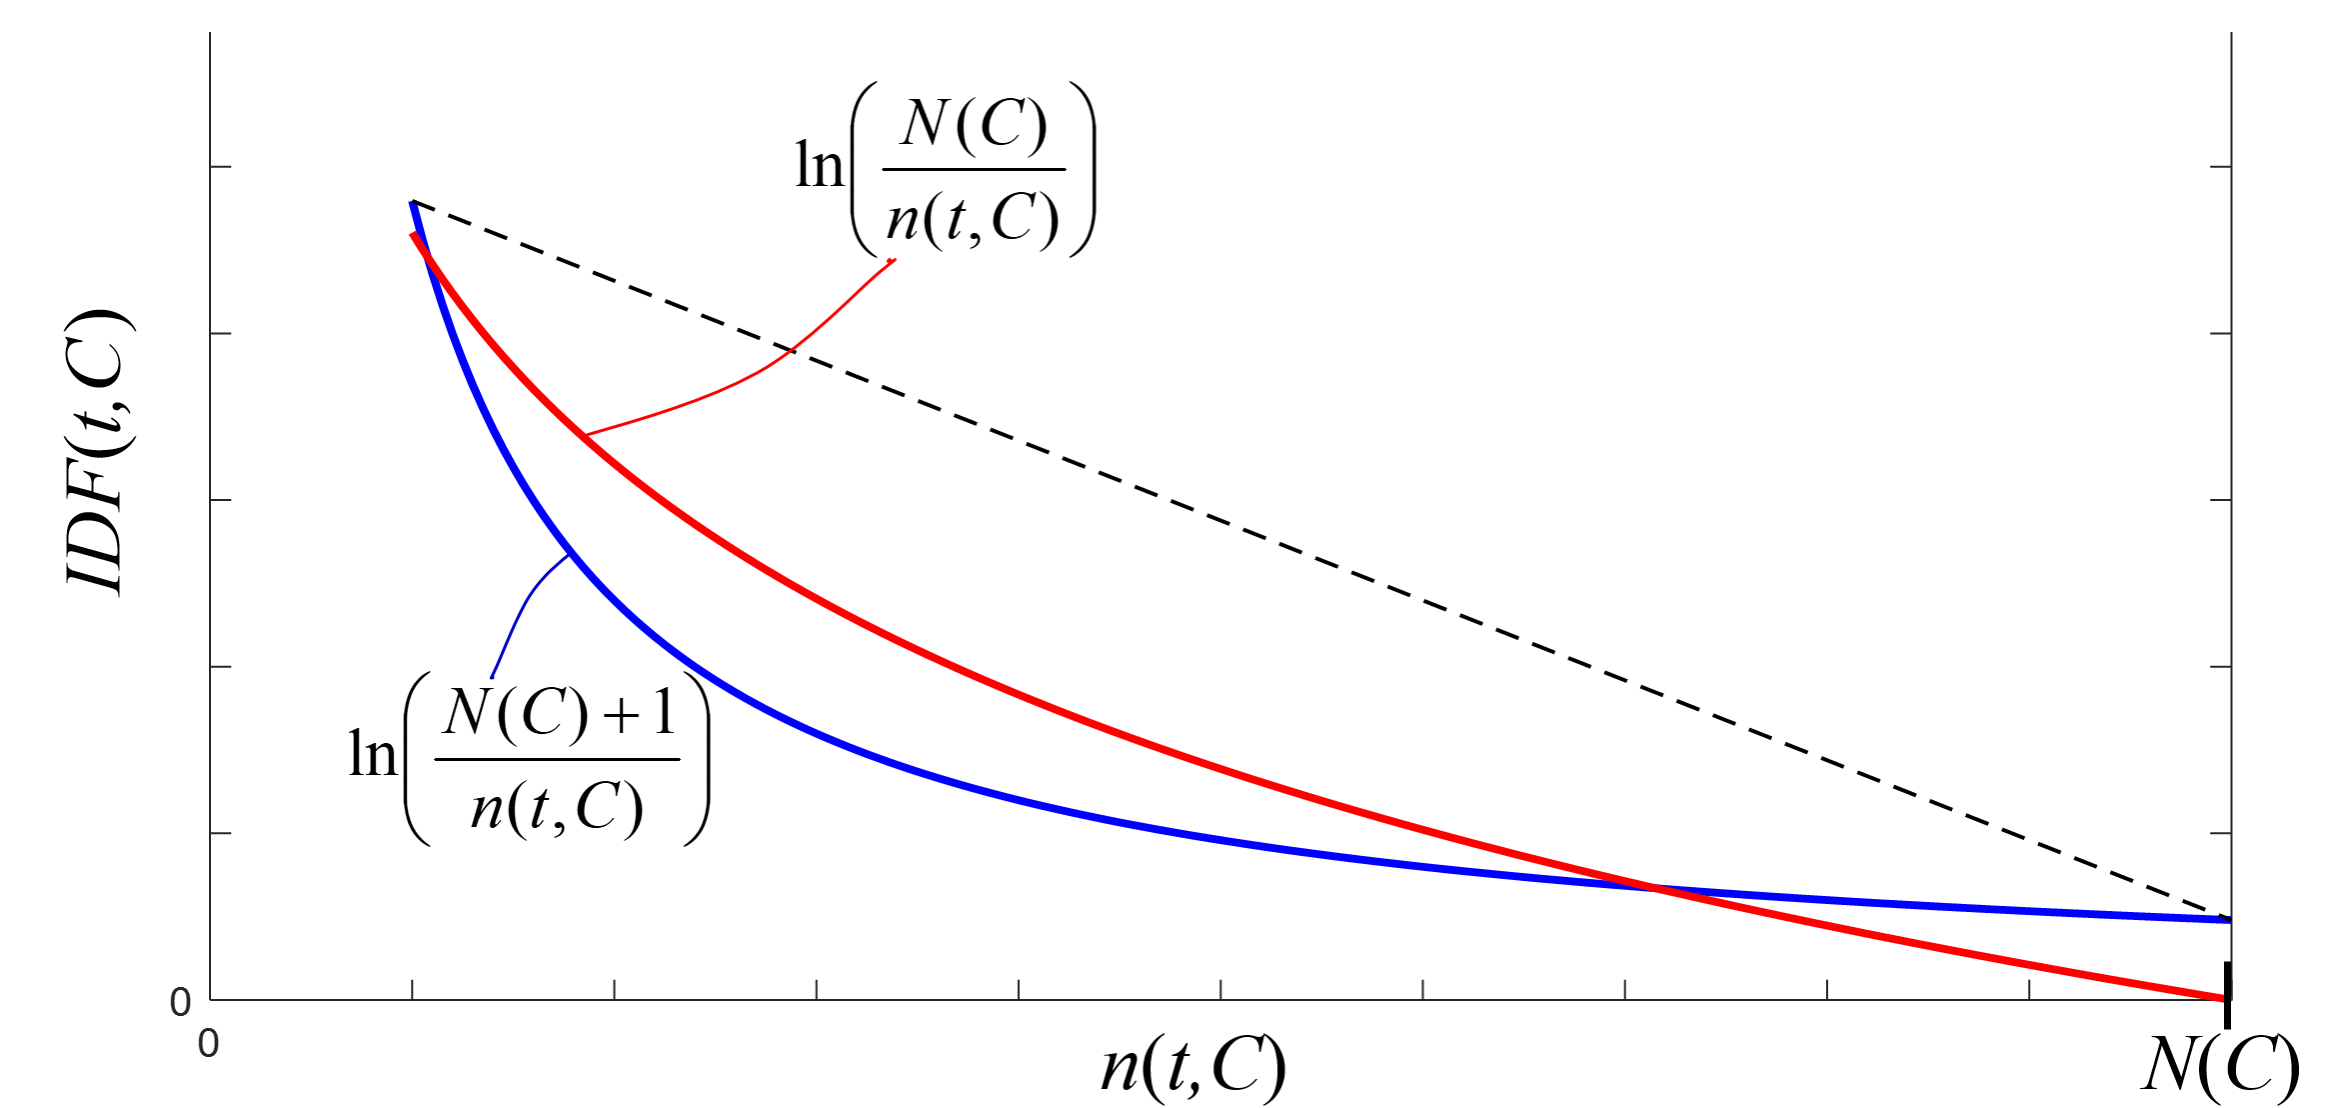
\includegraphics[width=0.6\linewidth]{img/popular_terms_penalty}
	\caption{Popular terms are penalised}
	\label{fig:populartermspenalty}
\end{figure}

\subsection{TF-IDF}
\begin{equation*}
	\text{TF-IDF}_{word} = \text{TF}_{word,doc}\cdot\text{IDF}_{word,coll}
\end{equation*}
Increases with the number of word occurrences within a document and the rarity of the word in the collection. Ranking of documents for a query is done by
\begin{equation*}
	\text{Score}_{query,doc} = \underset{word\in query\cap doc}{\sum} \text{TF-IDF}_{word,doc,coll}
\end{equation*}
\begin{minipage}{\textwidth}
	\renewcommand{\arraystretch}{1.5}
	\begin{tabularx}{\linewidth}{|l|X|p{2cm}|l|X|}
		\cline{1-2}\cline{4-5}
		& TF weights & & & IDF weights\\
		\cline{1-2}\cline{4-5}
		Binary & $ 0 / 1$& & Unary & 1\\
		\cline{1-2}\cline{4-5}
		Counts & $c(t,d)$ & & IDF & $\log\left(\frac{N(C)}{n(t,C)}\right)$\\
		\cline{1-2}\cline{4-5}
		Frequency & $\frac{c(t,d)}{\sum_{\tau\in d} c(\tau,d)}$ & & IDF.
		* & $ 1 + \log\left(\frac{N(C)}{n(t,C)}\right) $ \\
		\cline{1-2}\cline{4-5}
		Log Counts & $ 1 + \log\left( c(t,d) \right) $ & & IDF Smoothed & $\log\left(\frac{N(C)}{1 + n(t,C)}\right)$\\
		\cline{1-2}\cline{4-5}
		\vdots & \vdots & & \vdots & \vdots\\
		\cline{1-2}\cline{4-5}
	\end{tabularx}
\end{minipage}

\subsection{Document Length Normalisation}
Penalise long documents with a document length normaliser, as long documents have a better chance to match any query and are thus less specific. But avoid over-penalisation as documents can be long since they use more words, which should result in more penalisation, or as they have more content, which should be less penalised.
\begin{figure}[H]
	\centering
	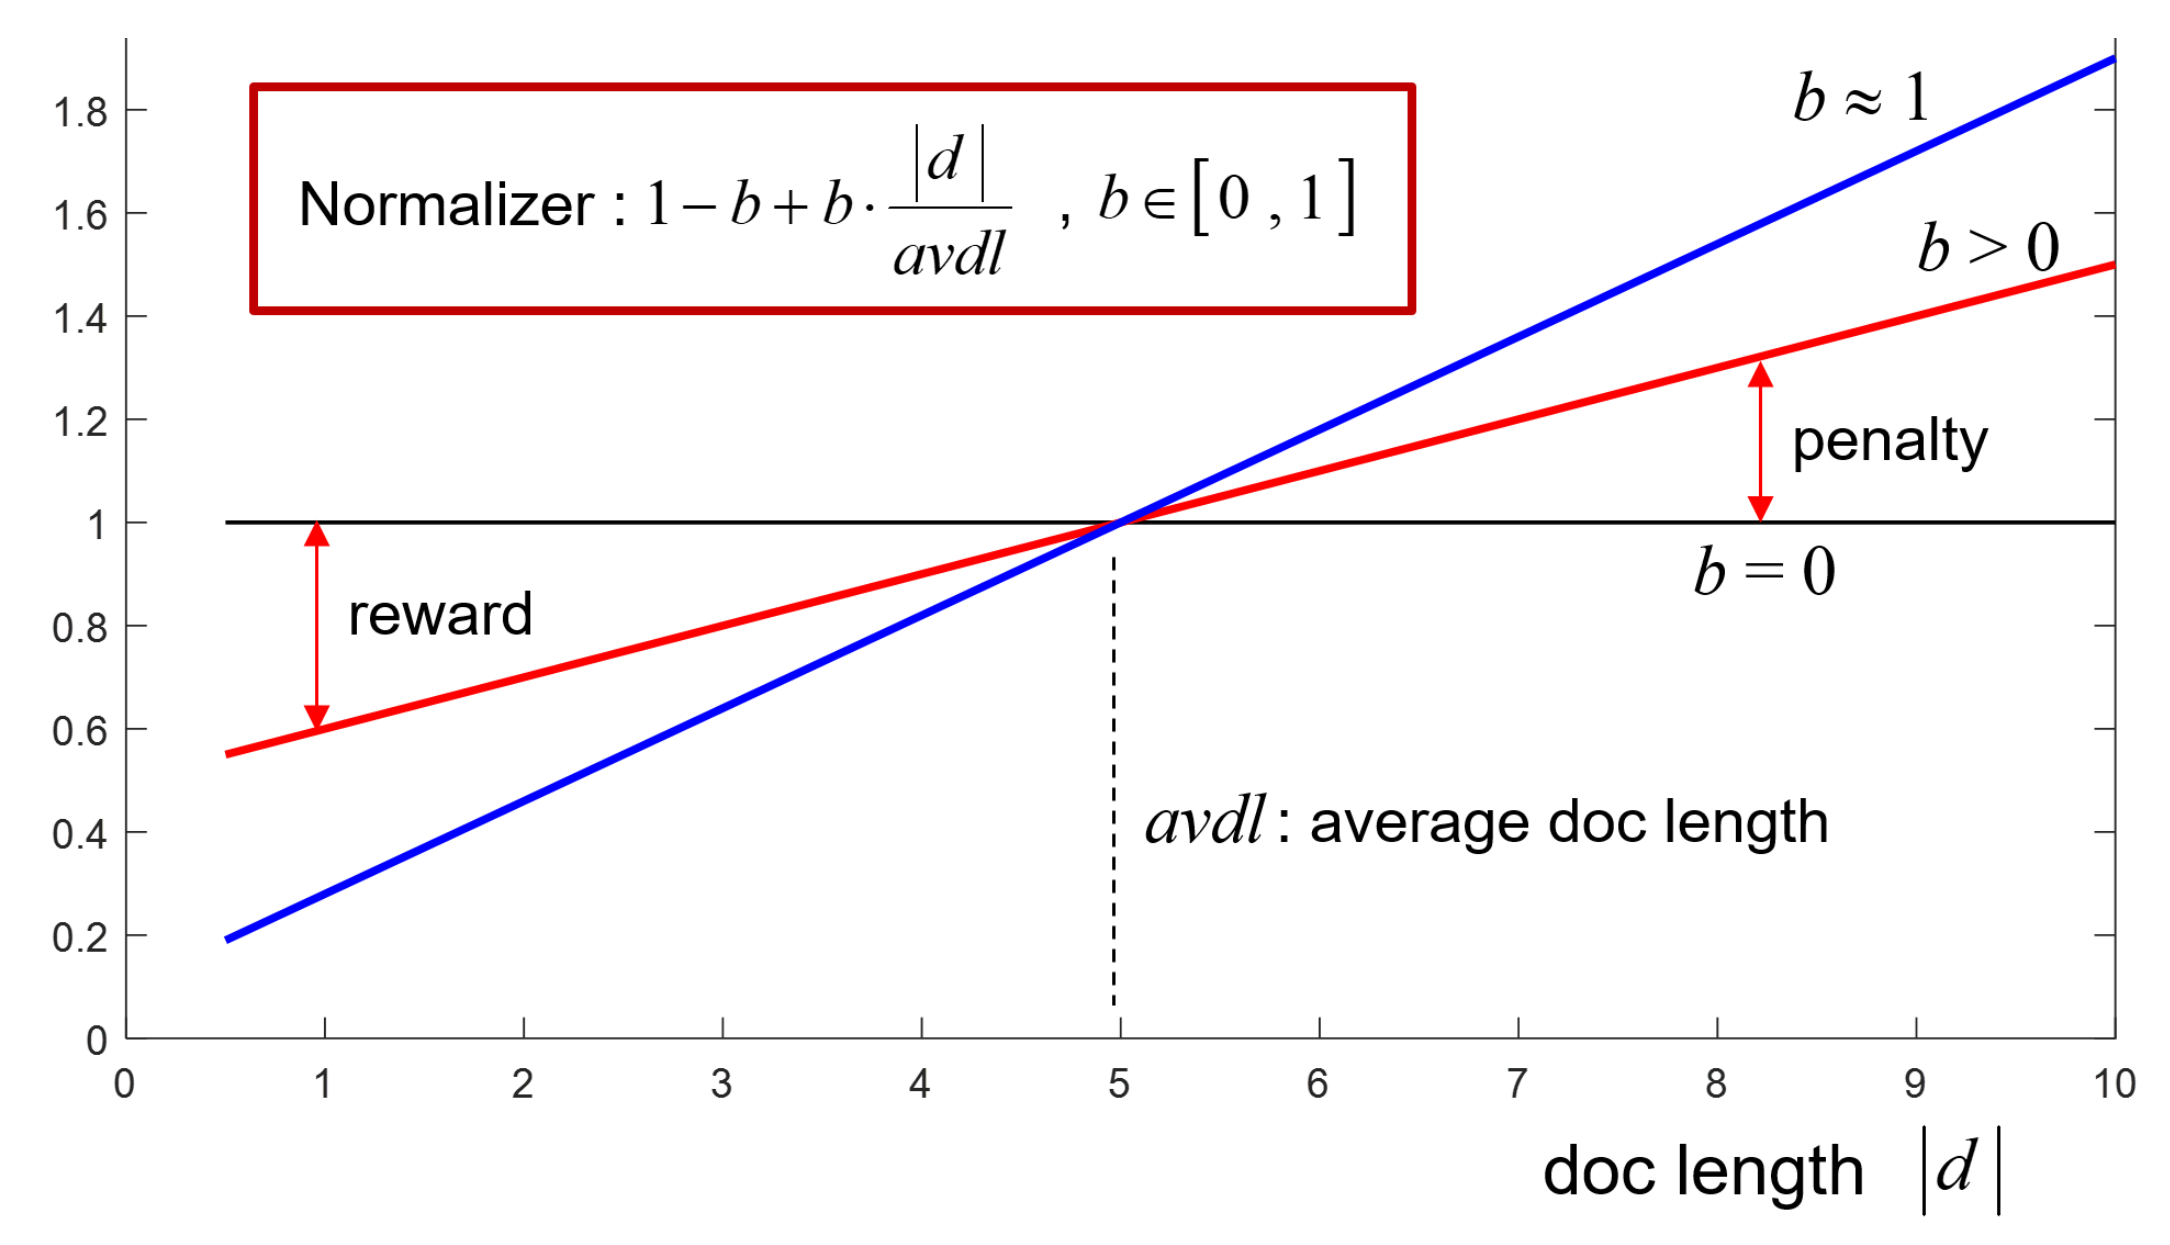
\includegraphics[width=0.6\linewidth]{img/pivot_length_normaliser}
	\caption{Average document length is used as a pivot point}
	\label{fig:pivotlengthnormaliser}
\end{figure}

\subsubsection{State of The Art Okapi BM25+}
Given a Query $Q$ containing keywords $q_1,\dots,q_n$, document $D$'s score is
\begin{equation*}
	\text{score}(D,Q) = \sum_{i=1}^{n}\text{IDF}(q_i) \cdot \left[ \frac{f(q_i,D)\cdot (k_1 + 1)}{f(q_i, D) + k_1\cdot\left( 1 - b + b\cdot\frac{\abs{D}}{\text{avgdl}} \right)} + \delta \right]
\end{equation*}
\begin{equation*}
	\text{IDF}(q_i) = \log \frac{N - n(q_i) + 0.5}{n(q_i) + 0.5}
\end{equation*}
\begin{itemize}[leftmargin=*, labelindent=2cm, labelsep=1cm, noitemsep,nosep]
	\item[$f(q_i,D)$] Term frequency of $q_i$ in document $D$
	\item[$\abs{D}$] length of document $D$
	\item[avgdl] average document length over corpus
	\item[$\delta$] free parameter, default $\delta = 1.0$
	\item[$k_1$] free parameter, $k_1 \in [1.2, 2.0]$
	\item[$b$] free parameter, default $b = 0.75$
	\item[$N$] number of documents in corpus
	\item[$n(q_i)$] number of documents containing $q_i$
\end{itemize}

\subsection{Vector Space Model}
Used to correlate words, sentences and documents by semantic similarity.
\begin{center}
	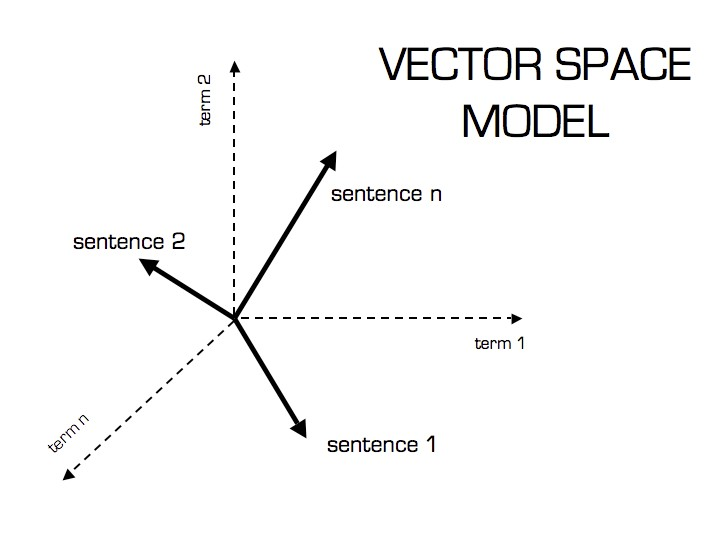
\includegraphics[width=0.5\linewidth]{img/vector_space_model}
\end{center}
For scoring the cosine similarity between documents and a query vector is preferred over the euclidean distance
\begin{itemize}[leftmargin=*, labelindent=3cm, labelsep=1cm, noitemsep]
	\item[similar scores] score vectors are in the same direction, angle between them is almost zero making the cosine lying near one or 100\%
	\item[unrelated scores] score vectors are nearly orthogonal and the cosine is thus near zero
	\item[opposite scores] score vectors in opposite directions, cosine is near minus one or -100\%
\end{itemize}         
The cosine similarity is calculated by
\begin{equation*}
	\cos(d_j,q) = \frac{\bm{d_j}\cdot \bm{q}}{\norm{\bm{d_j}}\norm{\bm{q}}} = \frac{\sum_{i=1}^{N} w_{i,j} w_{i,q} }{\sqrt{\sum_{i=1}^{N}w_{i,j}^2}\sqrt{\sum_{i=1}^{N}w_{i,q}^2}}
\end{equation*}
$\text{L}^2$ norm (Euclidean norm) is the square root of the dot product of the vector $\bm{p}$ with itself, and scales a vector to its unit-length
\begin{equation*}
	\norm{\bm{p}} = \sqrt{p_1^2 + p_2^2 + \dots + p_n^2} = \sqrt{\bm{p}\cdot\bm{p}}
\end{equation*}
Normalising all vectors to unit vectors this way allows for the dot-product to measure similarity, and do it in a more efficient way than cosine similarity. The dot product between two vectors $\bm{d_j}$ and $\bm{q}$ is high if $w_{ij}$ and $w_{iq}$ have similar characteristics, and is equivalent to the cosine similarity if the vectors are normalised.

\section{Word Embeddings}
An embedding is a \textbf{representation of words as dense vectors} such that the properties of the words and the relationships between the words are preserved. \textbf{Count-based methods} compute statistics of word co-occurrence in large text corpora, and then map these count-statistics down to a small, dense vector for each word. Predictive models use a (shallow) neural network to predict
words from its neighbours. The learned weights act as word vector representations.

Word embeddings are automatically learned and allow for vector-oriented reasoning based on the offsets between words.

\subsection{Context-Counting Word Vectors}
Represent mutual information of a word with other words by global co-occurrence counts using a pre-defined window size.
\begin{center}
	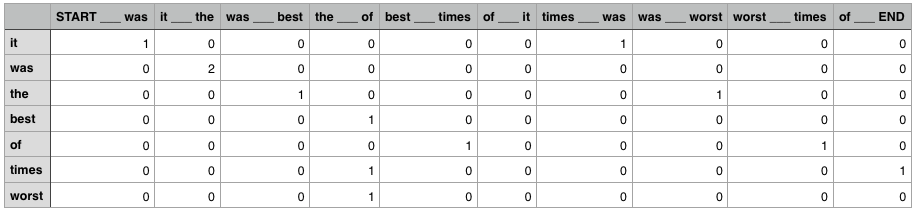
\includegraphics[width=0.8\linewidth]{img/context_counting}
\end{center}
The problem is that this matrix increases with vocabulary and windows size, which results in a very high dimensional, but sparse feature matrix. Use single value decomposition (SVD) to project the co-occurrence matrix to smaller dimension and take the sub-matrix as the word embedding matrix.

\subsection{Word2Vec}
Word2Vec is a simple and computationally efficient way to learn embeddings. It is a prediction based method and comes in two flavours, the Continuous Bag of Words (CBOW) and the Skip-gram model.
\begin{center}
	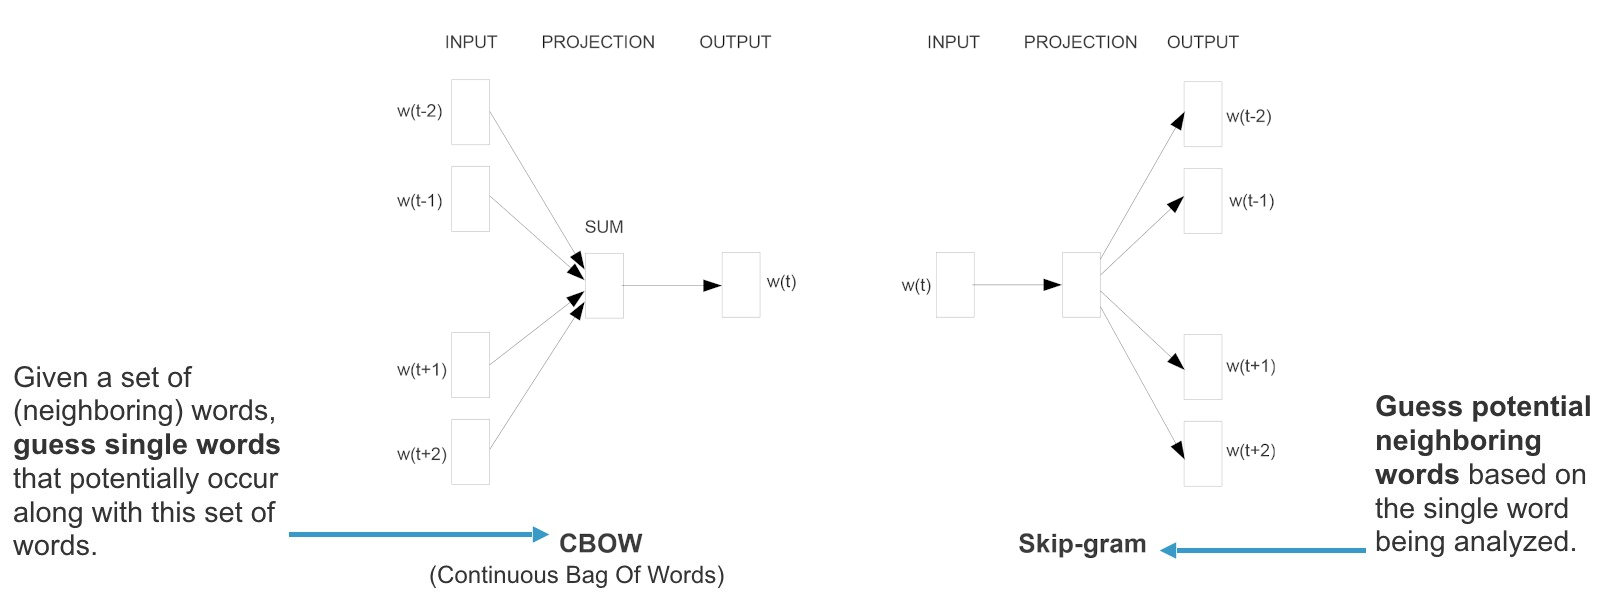
\includegraphics[width=0.8\linewidth]{img/word2vec_model}
\end{center}

\subsubsection{CBOW}
\begin{minipage}{0.5\linewidth}
	Given a set of context words, predict the centre word that potentially occurs with the context words. The input are $m$ one-hot vectors of context window words.
	\vspace{5em}
\end{minipage}
\begin{minipage}{0.5\linewidth}
	\begin{center}
		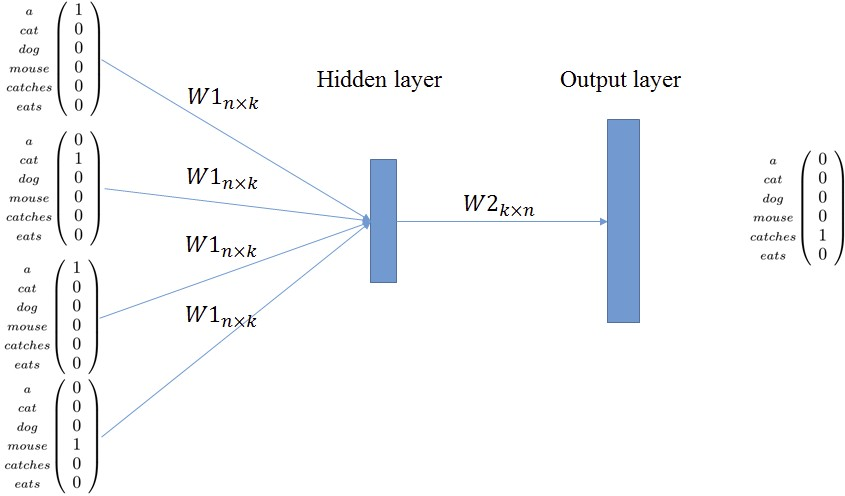
\includegraphics[width=0.9\linewidth]{img/word2vec_cbow}
	\end{center}
\end{minipage}

\subsubsection{Skip-Gram}
\begin{minipage}{0.6\linewidth}
	Given a center word, predict context words that potentially occur with 	the centre word. Input is the one-hot vector for word $w$.
	\vspace{10em}
\end{minipage}
\begin{minipage}{0.4\linewidth}
\begin{figure}[H]
	\centering
	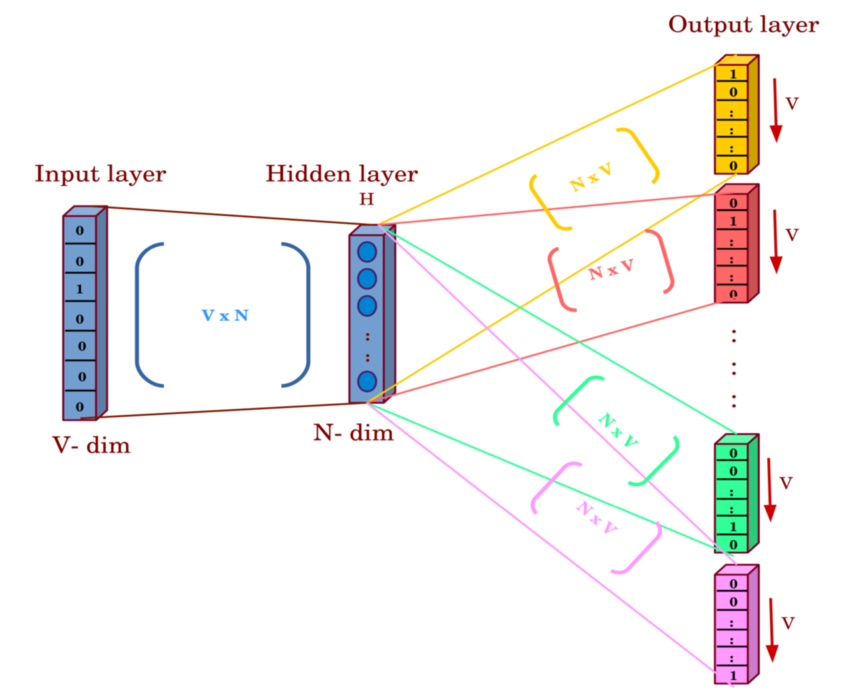
\includegraphics[width=0.9\linewidth]{img/word2vec_skip-gram}
	\caption{Source: \href{https://inspirehep.net/literature/1630982}{An Information Retrieval and Recommendation System for Astronomical Observatories}}
	\label{fig:word2vecskip-gram}
\end{figure}
\end{minipage}
\begin{center}
	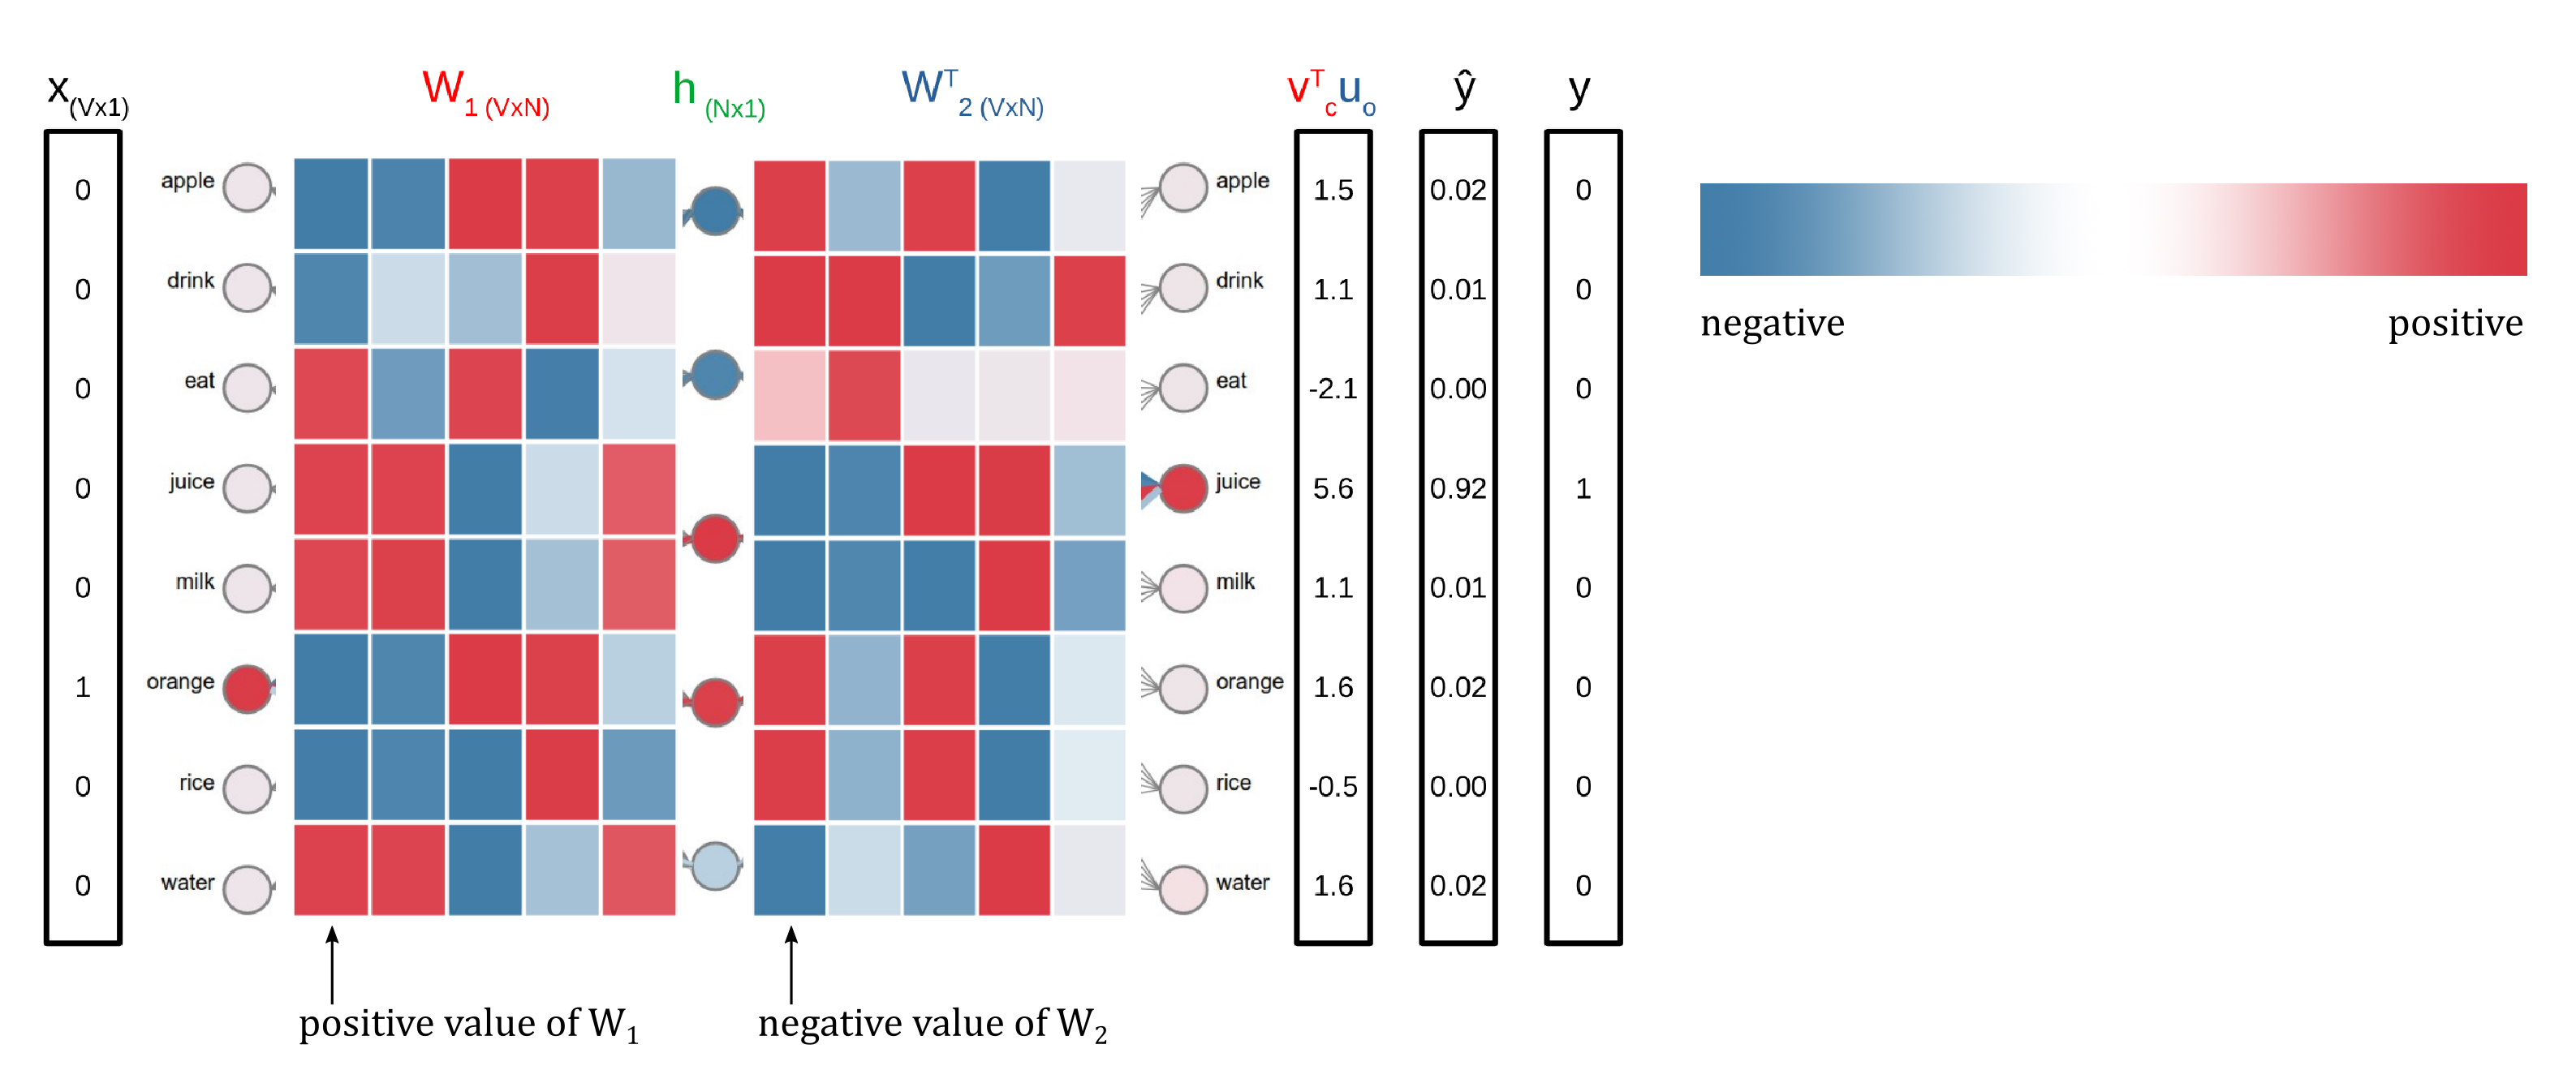
\includegraphics[width=0.9\linewidth]{img/word2vec_example}
\end{center}

\subsubsection{Softmax}
\begin{equation*}
	\hat{y} = p({\color{SteelBlue4}o}|{\color{red}c}) = \frac{e^{{\color{red}v_c^T}{\color{SteelBlue4} u_0}}}{{\color{SpringGreen4}\sum_{w\in V}} e^{{\color{red}v_c^T}{\color{SteelBlue4} u}_{\color{SpringGreen4} w}}}
\end{equation*}
Inner product ${\color{red}v_c^T}{\color{SteelBlue4} u_0}$
\begin{itemize}[label=-]
	\item ${\color{red}v_c^T}$ := embedding of word $w$ if word is {\color{red} center} word
	\item ${\color{SteelBlue4} u_0}$ := embedding of word $w$ if word is {\color{SteelBlue4} contex} word
	\item Measures the similarity of the two embedding representations of ${\color{red}v_c^T}$ and ${\color{SteelBlue4} u_0}$
\end{itemize}
The exponentiation makes all values positive and large values even larger, while the division by the {\color{SpringGreen4} sum over all words in the vocabulary} makes $\hat{y}$ a probability.

\subsection{GloVe}
Combines count based co-occurrence statistics with predictive context window method. GloVe is faster to train than Word2Vec and scales to huge corpora.

\subsubsection{Out of Vocabulary Words}
While using Word2Vec or GloVe out-of-vocabulary words will be encountered, as the possible vocabulary is infinitely large. Subword methods are based on the assumption that the semantic representation can be reconstructed from known parts of an unknown word.

FastText is an open-source, free, lightweight library that allows users to learn text representations and text classifiers. Each word is represented with a bag of $n$-grams in addition to the
word itself. It has proven to be more accurate than Word2Vec, but models are quite big and require a lot of computation for training.

\subsection{Practical Advice}
Use pre-trained word embeddings, unless there is a corpus of billions of words in the training set, where it is appropriate to start randomised. If your training set is small do not fine-tune the word embeddings. If the training set is large (more than one million words or with domain specific content), it probably will work better when fine-tuned to the task. It is generally advisable to compare results for both methods.

\section{Word Sense Disambiguation}

\subsection{Homonyms}
\begin{itemize}[leftmargin=*, labelindent=2cm, labelsep=1cm]
	\item[Homographs] words written the same way
	\item[Homophones] words that sound the same
\end{itemize}
In general Homographs cause problems with machine translation, while Homophones cause problems with text-to-speech. Words exhibiting these characteristics are called polysemous; words with multiple related senses.

\subsubsection{Zeugma Test}
Apply a word to two others in different senses and test if it makes sense.

"Routers are used to cut channels in wood and to connect different networks."

\subsection{Synonyms and Antonyms}
Synonyms are lexical items that have the same meaning in some or all contexts. Perfect synonymy seldom occurs, one or a few lexemes are typically preferable to other synonyms, and may convey the intended meaning better. This could be notions of politeness, register, acceptability, convention or nuance.

For example \textit{automobile} is more formal than \textit{car}.

\vspace{1em}
\noindent
Antonyms are words with opposite senses
\begin{itemize}[leftmargin=*, labelindent=4cm, labelsep=1cm]
	\item[Reversives] rise/fall, in/out, up/down
	\item[Opposite ends of a scale] long/short, hot/cold
\end{itemize}

\subsection{Hyponymy and Hypernymy}
One sense is a hyponym of another if it denotes a subclass. Sense A is a hyponym of sense B if being an A entails being a B.
\begin{itemize}[label=-]
	\item A:B = hyponym:hypernym = subtype:supertype
	\item Also known as the IS-A relationship
\end{itemize}
Hypernymy is the opposite relationship.

\subsection{Meronymy and Holonymy}
Part-whole and whole-part relationship. A meronym is a part of its holonym, for example a \textit{wheel} is a meronym of \textit{car}. There is a HAS-A relationship between a holonym and its meronym.

\subsection{Word Similarity Based on WordNet}
Look at the shortest path between sense nodes.
\begin{center}
	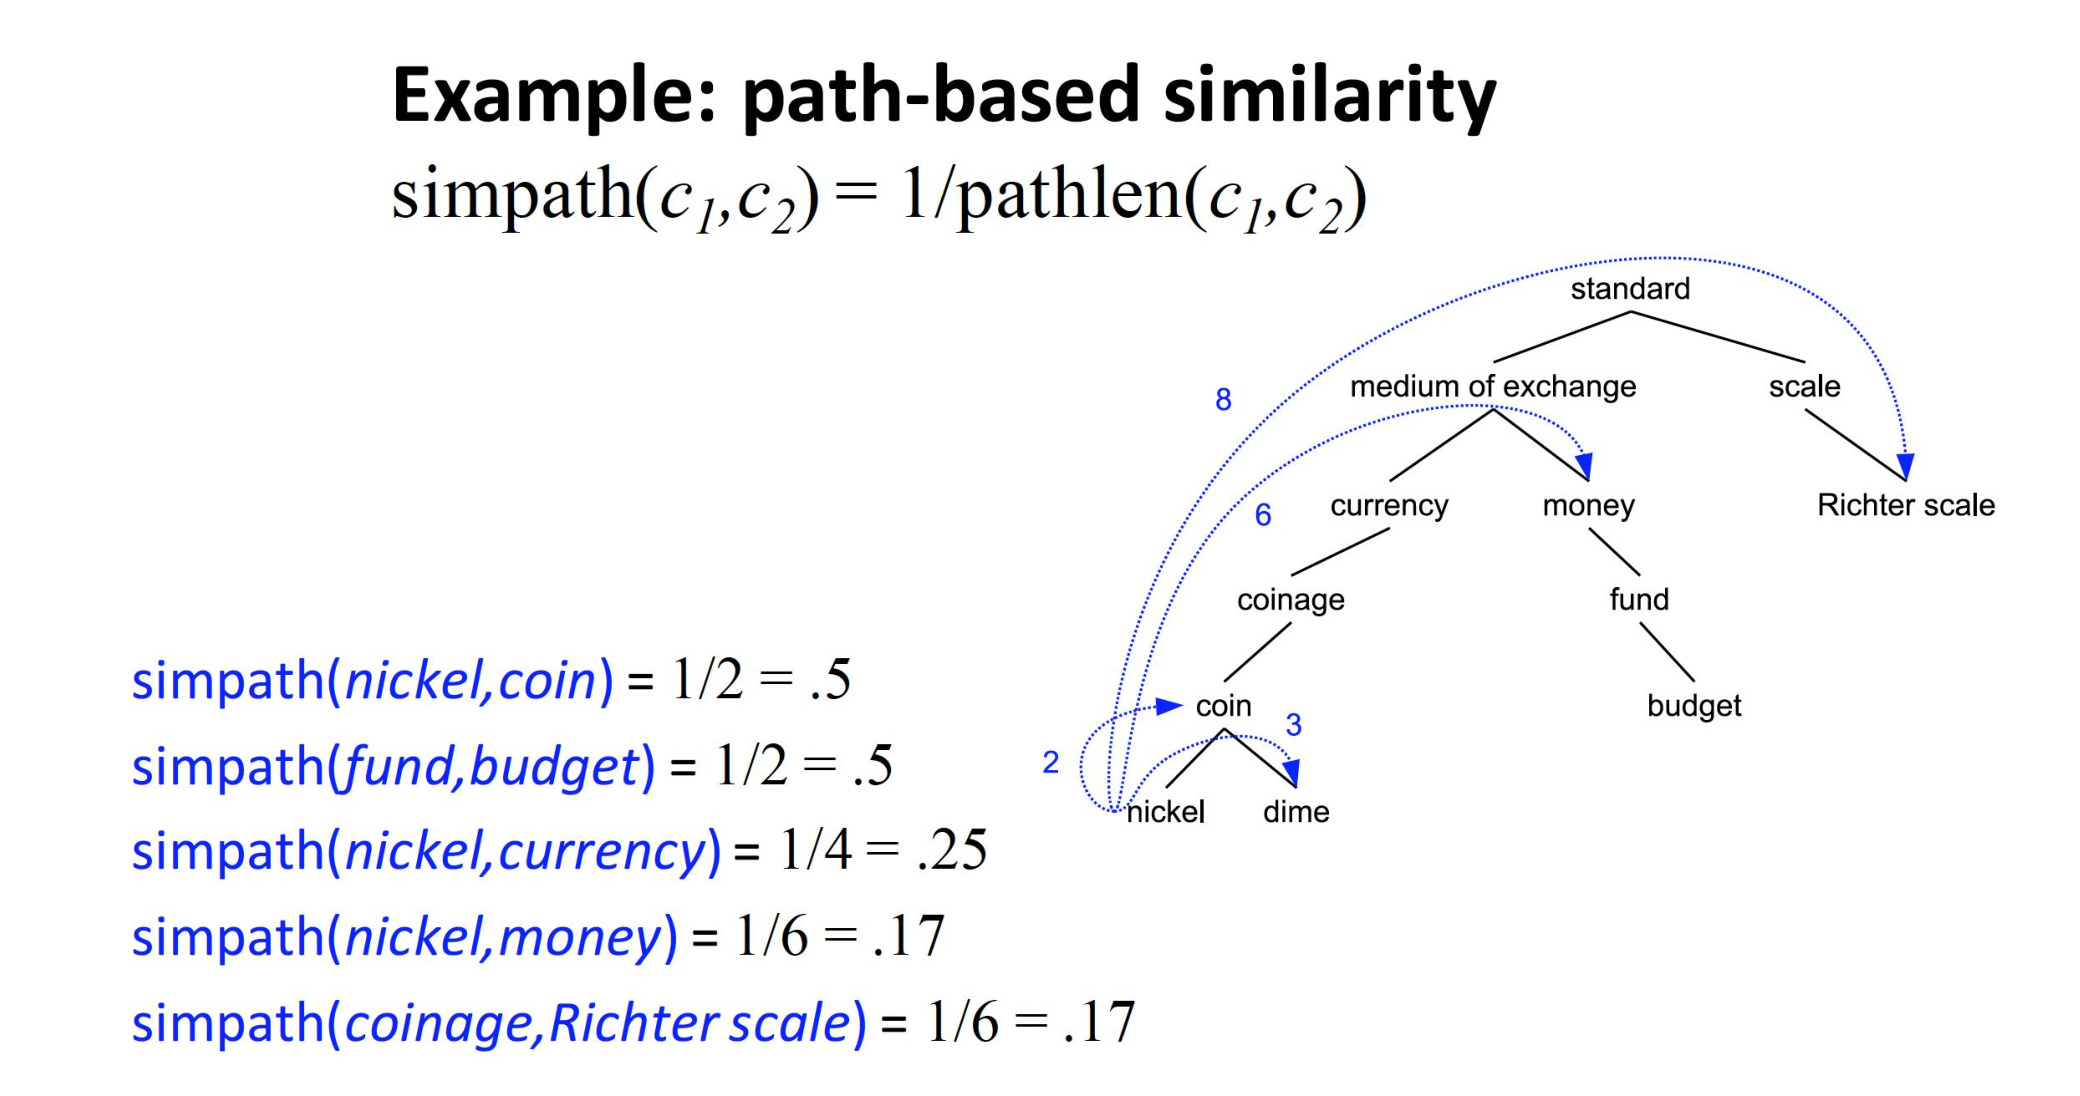
\includegraphics[width=0.8\linewidth]{img/WordNet_similarity}
\end{center}

\subsection{Word Vectors and Word Meaning}
\begin{itemize}
	\item One-hot vectors: No notion of word meaning
	\item Co-occurence matrices: words are represented by the weighted occurrence of other words in their context
	\item Pointwise mutual information (PMI) matrices: each element $(i,j)$ signifies whether words $i$ and $j$ are more likely to occur jointly than to be independent
	\begin{itemize}
		\item Negative PMI tends to be unreliable, as words co-occur less than expected with a corpus too small
		\item In practice positive PMI (PPMI) is used
	\end{itemize}
\end{itemize}
\begin{equation*}
	\text{PPMI}(w_1,w_2) = \max{\left(\log_2{\left(\frac{P(w_1,w_2)}{P(w_1)P(w_2)}\right)}\right)}
\end{equation*}

\subsection{Word Sense Disambiguation}
\textbf{Extrinsic} evaluation
\begin{itemize}
	\item Embed WSD in another task
	\item Measure the task performance without and with WSD and see whether it improves
\end{itemize}
\textbf{Intrinsic} evaluation
\begin{itemize}
	\item Use a labeled corpus
	\item Measure the accuracy, evaluated based on held-out data from the labeled corpus
\end{itemize}
As a baseline choose the most frequent sense or use the Lesk Algorithm.

\subsubsection{Simplified Lesk Algorithm}
The principle is to choose sense with most word overlap between gloss and context. Disambiguate the word bank in the sentence:

"The bank can guarantee that deposits will eventually cover future tuition costs because it invests in adjustable-rate mortgage securities."

\begin{center}
	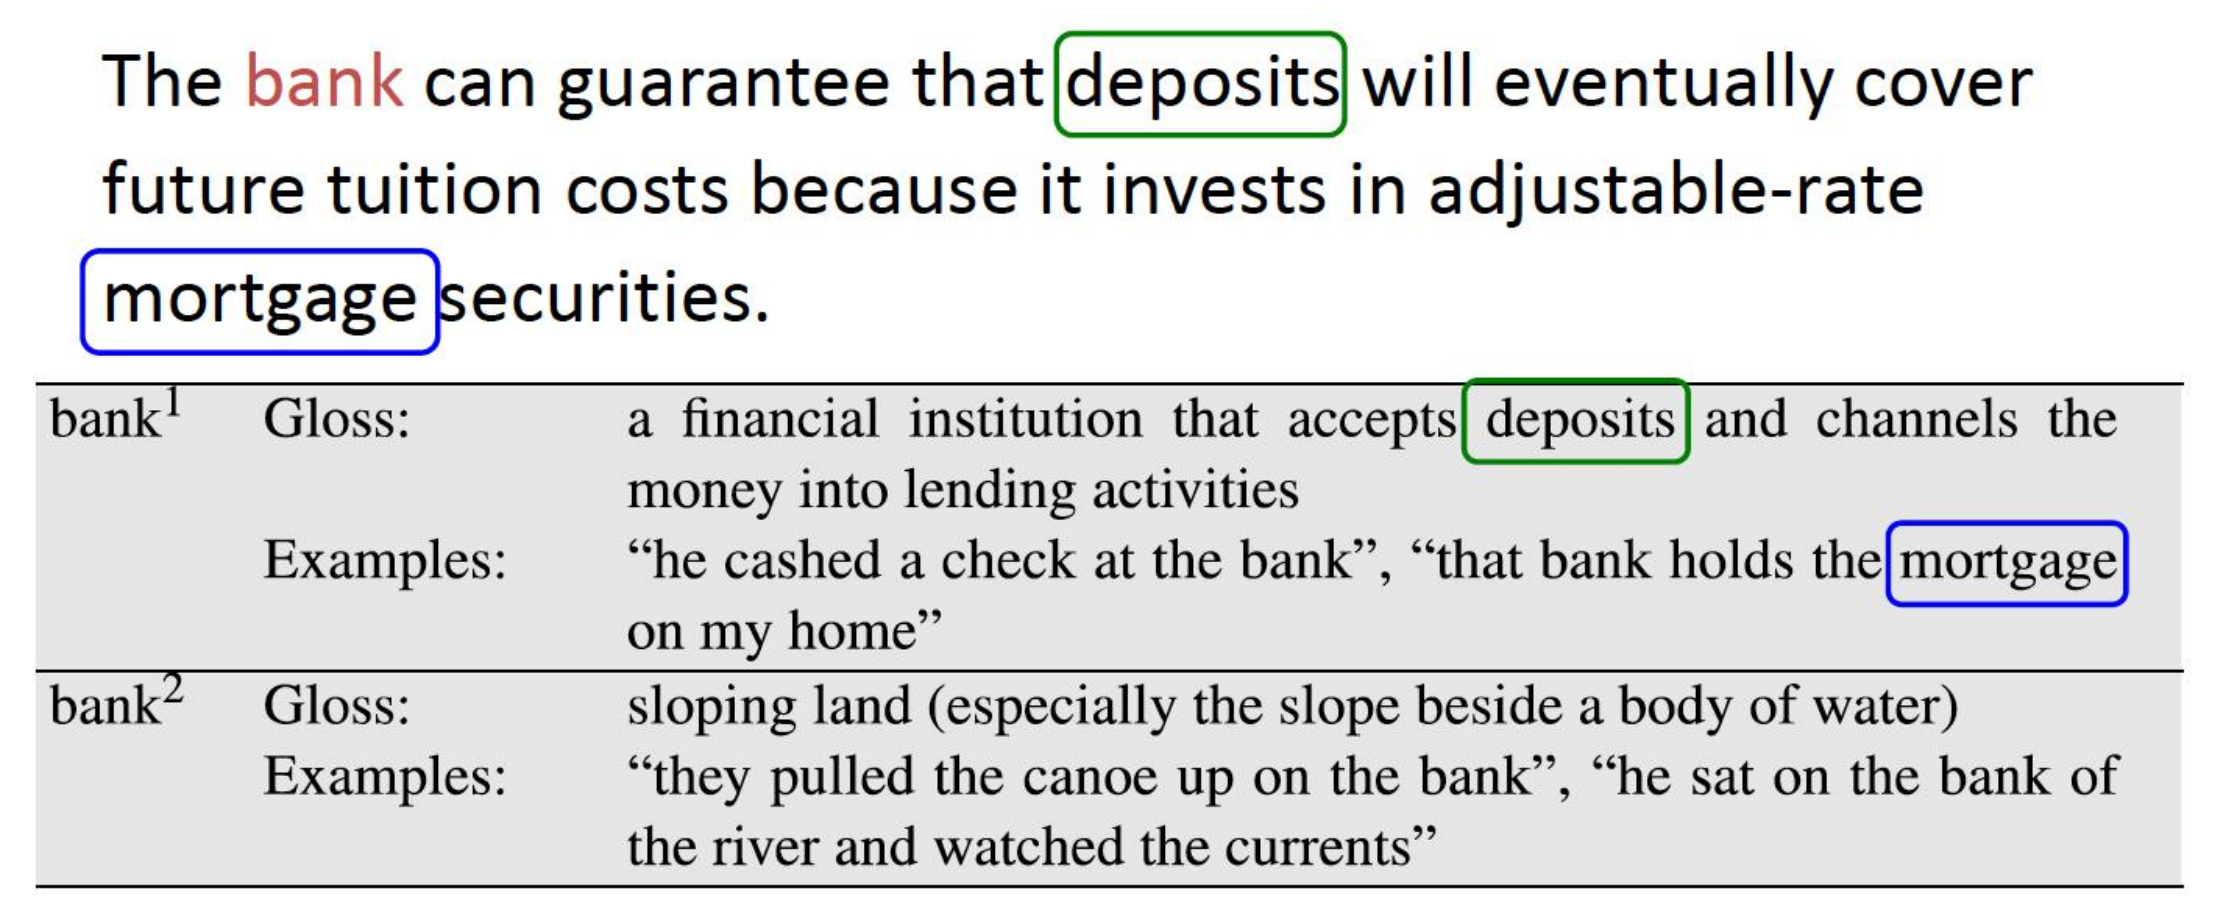
\includegraphics[width=0.7\linewidth]{img/simplified_lesk_algorithm}
\end{center}

\subsubsection{Word Sense Disambiguation Based on Word Embeddings}
Embedding vectors like Word2Vec or GloVe can be used for word sense disambiguation.
\begin{itemize}
	\item Capture context of each word sense
	\begin{itemize}
		\item Find the gloss of the word sense in WordNet
		\item Get the embedding vectors of the words in the gloss
		\item Average out the embedding vectors and obtain an embedding vector for the context of each target word sense
	\end{itemize}
	\item Do the same for the sentence containing the target word
	\item Compare the embedding vector  for the target sentence to the embedding vectors for the target word senses
	\item Pick the word sense whose embedding vector is the most similar to the one of the target sentence
\end{itemize}

\begin{minted}[linenos]{python}
for sense in range (1, len(word_vectors)):
	print ('context '+ str(sense) + ': ' + get_gloss(target_word, sense)) 
\end{minted}
\begin{minted}[breaklines]{text}
context 1: sloping land (especially the slope beside a body of water) 
context 2: a financial institution that accepts deposits and channels the money into lending activities 
context 3: a long ridge or pile 
context 4: an arrangement of similar objects in a row or in tiers 
context 5: a supply or stock held in reserve for future use (especially i n emergencies) 
context 6: the funds held by a gambling house or the dealer in some gambl ing games 
context 7: a slope in the turn of a road or track; the outside is higher than the inside in order to reduce the effects of centrifugal force 
context 8: a container (usually with a slot in the top) for keeping money at home 
context 9: a building in which the business of banking transacted 
context 10: a flight maneuver; aircraft tips laterally about its longitud inal axis (especially in turning) 
\end{minted}

\section{Part-of-Speech Tagging}
PoS tagging means identifying the grammatical category of each word token.

\vspace{1em}
\noindent
\begin{minipage}{0.5\linewidth}
	\begin{itemize}
		\item nouns
		\item verbs
		\item adjectives
		\item adverbs
		\item preposition
	\end{itemize}
\end{minipage}
\begin{minipage}{0.5\linewidth}
	\begin{itemize}
		\item particles
		\item conjunctions
		\item pronouns
		\item numerals
		\item interjections
	\end{itemize}
\end{minipage}

\subsection{Corpora}
There are corpora with manually tagged PoS, which are both in part in NLTK
\begin{itemize}
	\item Brown corpus
	\item Penn Treebank
\end{itemize}
The Penn Treebank tags are widely used for English language PoS tagging.

\noindent
\begin{minipage}[t][][t]{0.5\linewidth}
	\begin{tabularx}{\linewidth}{c|c|X}
		\textbf{Number} & \textbf{Tag} & \textbf{Description} \\
		\hline
		1 & CC & Coordinating conjunction \\
		2 & CD & Cardinal number \\
		3 & DT & Determiner \\
		4 & EX & Existential there \\
		5 & FW & Foreign word \\
		6 & IN & Preposition or subordinating conjunction \\
		7 & JJ & Adjective \\
		8 & JJR & Adjective, comparative \\
		9 & JJS & Adjective, superlative \\
		10 & LS & List item marker \\
		11 & MD & Modal \\
		12 & NN & Noun, singular or mass \\
		13 & NNS & Noun, plural \\
		14 & NNP & Proper noun, singular \\
		15 & NNPS & Proper noun, plural \\
		16 & PDT & Predeterminer \\
		17 & POS & Possessive ending \\
		18 & PRP & Personal pronoun \\
		19 & PRP\$ & Possessive pronoun
	\end{tabularx}
\end{minipage}
\begin{minipage}[t][][t]{0.5\linewidth}
	\begin{tabularx}{\linewidth}{c|c|X}
		\textbf{Number} & \textbf{Tag} & \textbf{Description} \\
		\hline
		20 & RB & Adverb \\
		21 & RBR & Adverb, comparative \\
		22 & RBS & Adverb, superlative \\
		23 & RP & Particle \\
		24 & SYM & Symbol \\
		25 & TO & to \\
		26 & UH & Interjection \\
		27 & VB & Verb, base form \\
		28 & VBD & Verb, past tense \\
		29 & VBG & Verb, gerund or present participle \\
		30 & VBN & Verb, past participle \\
		31 & VBP & Verb, non-3rd person singular present \\
		32 & VBZ & Verb, 3rd person singular present \\
		33 & WDT & Wh-determiner \\
		34 & WP & Wh-pronoun \\
		35 & WP\$ & Possessive wh-pronoun \\
		36 & WRB & Wh-adverb
	\end{tabularx}
\end{minipage}

\begin{figure}[H]
	\centering
	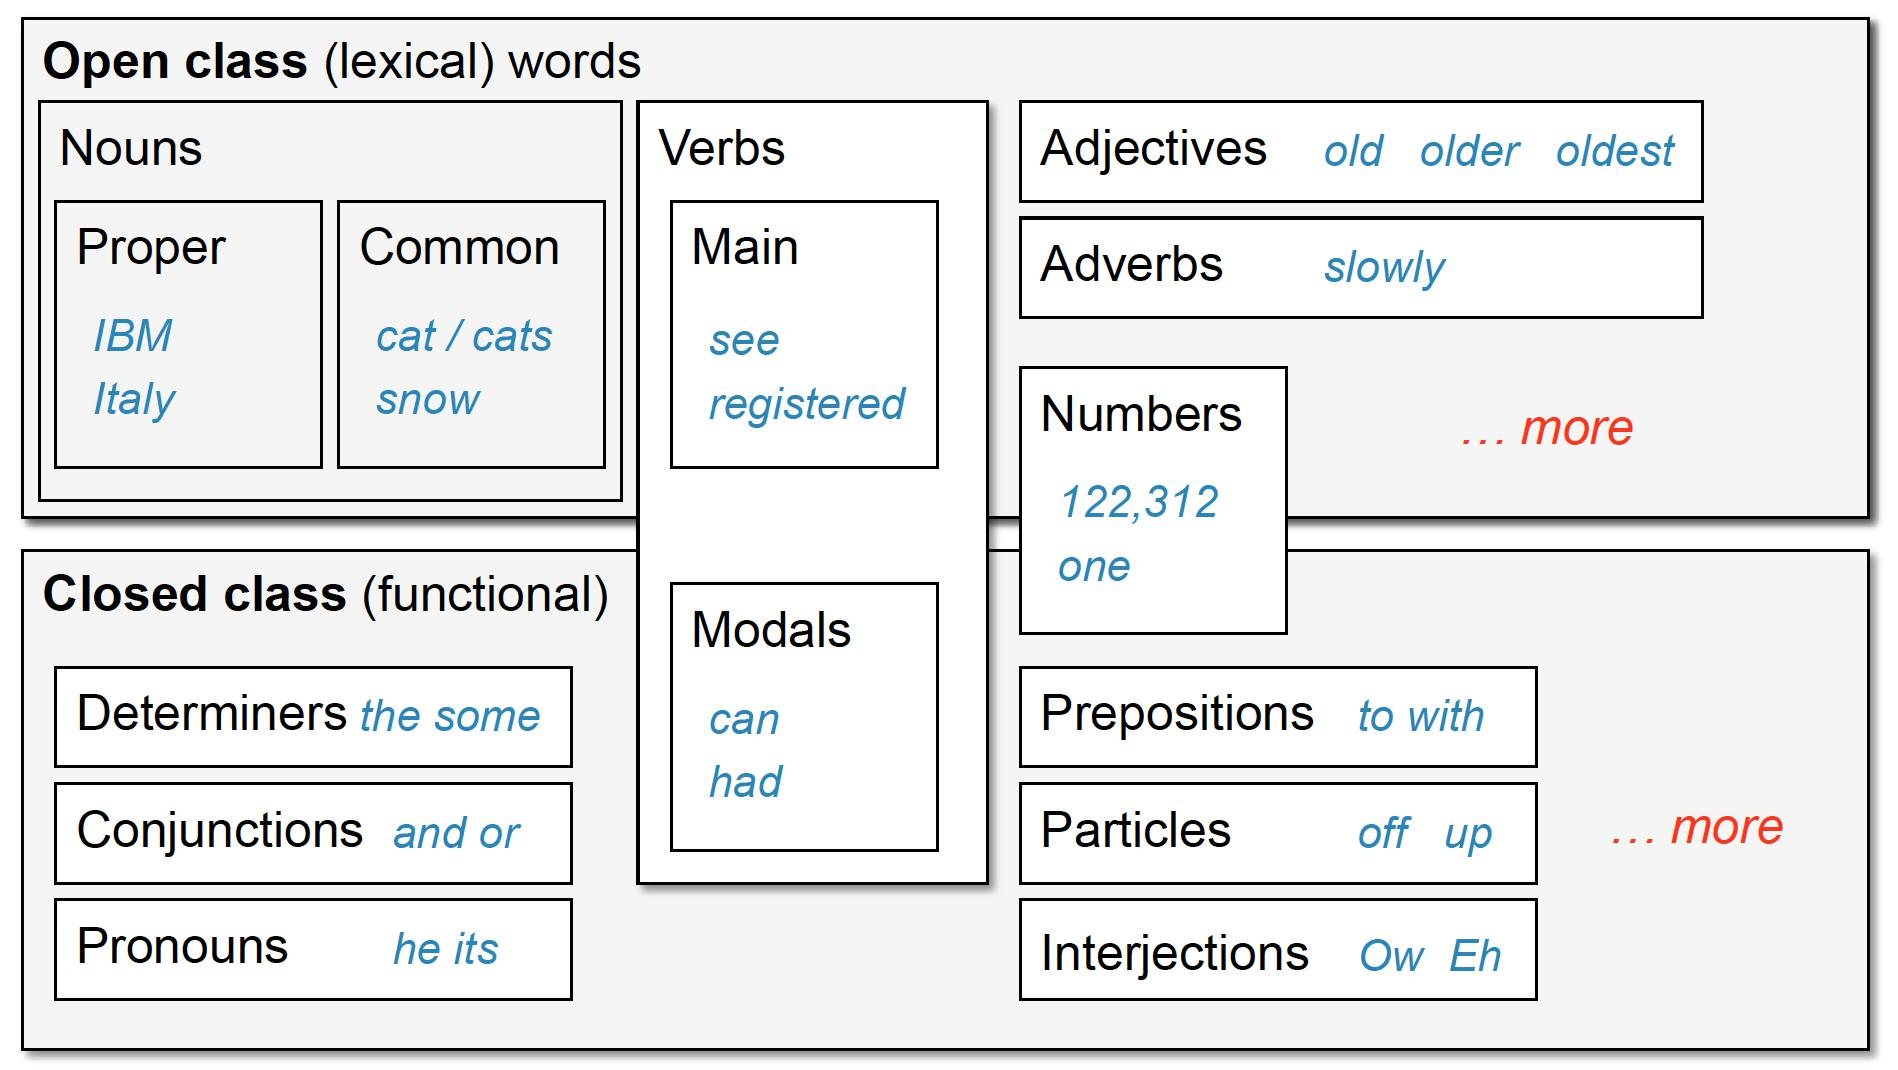
\includegraphics[width=0.9\linewidth]{img/open_close_classes}
	\caption{Open and closed classes}
	\label{fig:opencloseclasses}
\end{figure}

\subsection{English Nouns}
\begin{itemize}
	\item Count nouns allow for grammatical enumeration
	\item Mass nouns are used for a homogeneous group of concepts which are not countable
	\item Proper nouns are used to mane people, places or things, and are generally capitalised
\end{itemize}

\subsection{English Verbs}
\begin{itemize}
	\item Main verbs refer to actions and processes
	\item Auxiliary or Modal verbs change the meaning of main verbs
	\item There are four inflections
	\begin{itemize}
		\item Non-third person singular (VBP)
		\item Third person singular (VBZ)
		\item Progressive (VBG)
		\item Past participle (VBN)
	\end{itemize}
\end{itemize}

\subsection{Other English Part of Speech Components}
\begin{itemize}
	\item Adjectives characterise nouns
	\item Adverbs characterize verbs, adjectives, other adverbs, or word groups, they are separated into directional, degree, manner or temporal adverbs
	\item Prepositions specify relationships, be that spatial, temporal or agency\\
	\emph{arrive at the theater on time}
	\item Particles look like prepositions or adverbs but serve to modify the meaning of the verb that precedes them\\
	\emph{to find out}
	\item Determiners appear directly before a noun
	\begin{itemize}
		\item definite article: the
		\item indefinite article: a,an
		\item demonstratives: this, that, these, those
	\end{itemize}
	\item Conjunctions join clauses
	\begin{itemize}
		\item coordinating conjunctions link clauses of equal importance\\
		\emph{I respect his opinion but in this case he's factually wrong.}
		\item subordinating conjuctions a less important clause to complement a more important clause
	\end{itemize}
\end{itemize}

\subsection{Pronouns}
\begin{itemize}
	\item Relative pronouns introduce subordinate clauses that modify their antecedent
	\item Interrogative pronouns introduce questions
	\item Demonstrative pronouns identify or point at nouns
	\item Indefinite pronouns refer to nonspecific persons or things
\end{itemize}

\subsection{Handling Ambiguity}
For each ambiguous word token, choose the tag that is most frequent for that word token in the training corpus.
\begin{itemize}
	\item PRP+VBD is very common, while PRP+VBN is exceedingly uncommon
	\item RB+RB is very common, also at the end of a sentence
	\item RB+JJ is also very common, but not at the end of a sentence
	\item IN+JJ and IN+RB are both fine, but there would have to be more word tokens afterwards
\end{itemize}

\subsection{PoS Tagging as Sequence Classification}
A sentence is a sequence of observations, thus tagging can use probabilistic methods to choose the most likely tag sequence. In practice, each token is classified independently while using information about the surrounding tokens as input features. For ambiguous tags the forward and backward sequence of the already identified tags can be used.

\subsection{Markov Chains}
\textbf{Markov chains} are models that identify the underlying probabilities of a sequence of random variables.
\begin{itemize}
	\item a set of $N$ state variables
	\item a transition probability matrix $A$, where $a_{i,j}$ is the probability of going from state $i$ to state $j$
	\item an initial probability distribution over the $N$ states
	\begin{itemize}
		\item this is what is known \emph{a priori} before observing the system
		\item $\pi_i$ is the probability that the chain will start in state $i$
	\end{itemize}
\end{itemize}
A key assumption is that the next state only depends on the current state. For word sequences, this means that the assumption is that the next word only depends on the current word.

\begin{figure}[H]
	\centering
	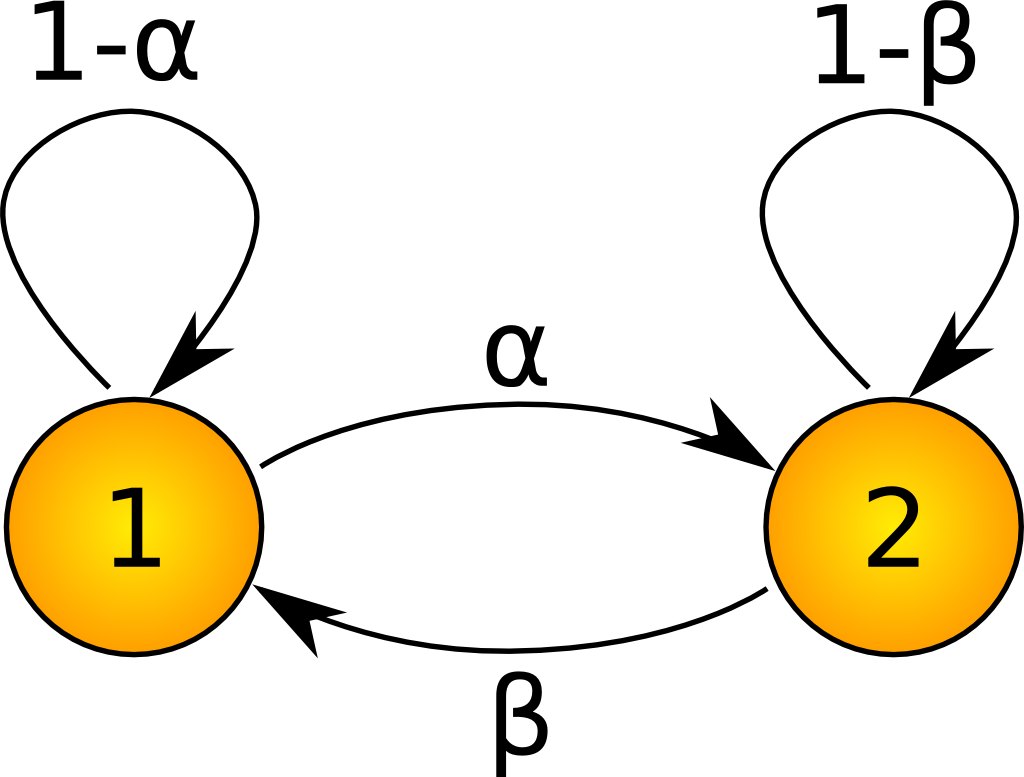
\includegraphics[width=0.4\linewidth]{img/two_state_markov_model.png}
	\caption{Two-state Markov Chain Model \parencite{markov}}
\end{figure}

Notice that the probabilities sum to one for each state ($ \alpha + (1-\alpha) = 1$). The transition matrix $A$ for this system is given by
\begin{equation*}
	\begin{pmatrix}
	1-\alpha & \alpha\\
	\beta & 1-\beta
	\end{pmatrix}
\end{equation*}
$n$ steps of a Discrete State Markov Chain (DSMC) can be simulated simply b y repeated multiplication of the transition matrix with itself.

Unfortunately Markov Chains only work if the interest lies in the probability of observed events. In PoS tagging, interest lies in the probability of things that can't be observed directly. Namely these are the tags, which are hidden. Fortunately \textbf{Hidden Markov Chains} enable the modelling of sequences with both observed events and related hidden events. In PoS tagging these correspond to words and tags.
\begin{itemize}
	\item a set of $N$ states
	\item a $N\times N$ \textbf{transition matrix} $A$ where $a_{i,j}$ is the probability of transitioning from state $i$ to state $j$
	\item a sequence $O$ of $T$ observations (drawn from a set of $V$ possible observations): $O = o_1, o_2, \dots, o_T$
	\item a $N\times V$ \textbf{emission matrix} $B$ where $b_{i,t} = P\left(o_t\middle| i\right)$ is the probability of state $i$ generating observation $o_t$
	\item an initial probability distribution over the $N$ states
\end{itemize}
Let $W$ be an observed word sequence and $T$ be a hidden tag sequence. The interest lies in $\hat{T}$ over all possible tag sequences.
\begin{equation*}
	\hat{T} = \arg\max P(T|W) =\arg\max P(W|T)P(T) = \arg\max \prod_{i} P\left( w_i \middle| t_i \right) \prod_{i} P\left( t_i \middle| t_{i-1} \right)
\end{equation*}
The process used to discover the tag sequence that maximizes $P(W|T)P(T)$ is called decoding and can be carried out using the Viterbi algorithm.

\subsection{Viterbi Algorithm for Hidden Markov Models}
The Hidden Markov Model may be represented as a graph called a trellis with a row for each tag and a column for each word
\begin{center}
	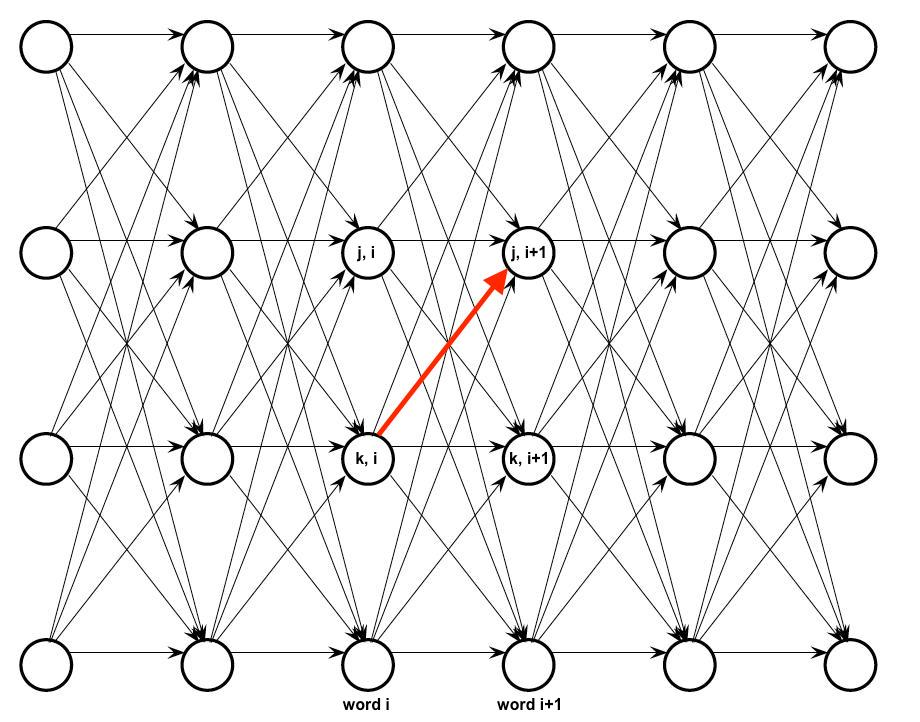
\includegraphics[width=0.5\linewidth]{img/vitrelli_trellis}
\end{center}
The $i$th column corresponds to the $i$th observation, the $k$th row corresponds to the $k$th hidden stage. The goal is to find the most probable path through the trellis, which refers to the path with the highest end-to-end probability computed as the products of the weights along the path.

The weight of the arrow from node $(k,i)$ to node $(j,i+1)$ is the product of two probabilities
\begin{itemize}[noitemsep,nosep]
	\item the probability of going from state $k$ to $j$\qquad $a_{k,j} = P(j|k)$
	\item the probability of state $j$ generating word $i+1$ \qquad $b_{j,i+} = P(i+1|j)$
\end{itemize}
The path through the trellis with the highest end-to-end probability is the most likely tag sequence associated to the word sequence.

\begin{center}
	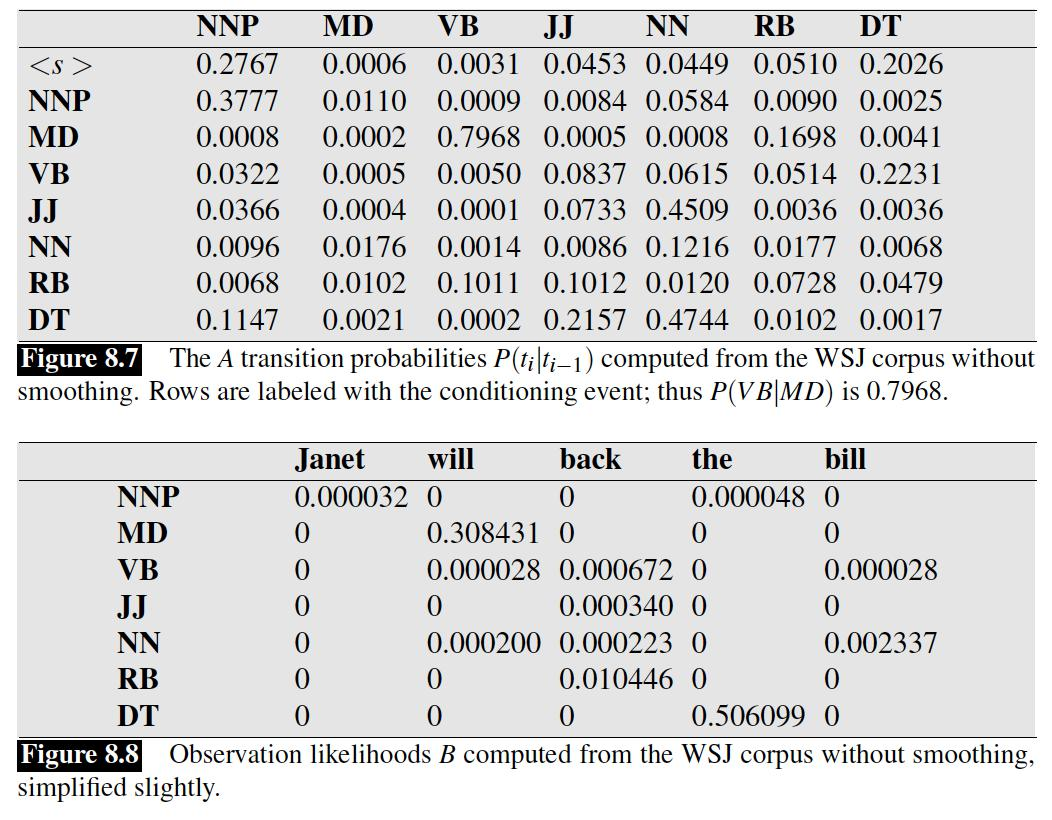
\includegraphics[width=0.6\linewidth]{img/vitrelli_trellis_example}
\end{center}

\section{Language Models}
Language modelling is the task of predicting what word follows a sequence of words. The formal definition is: given a sequence of words $w^{(1)}, w^{(2)},\dots, w^{(t-1)}$ a language model computes the probability distribution of the next word $w^{(t)}$
\begin{equation*}
	P\left(w^{(t)} \middle| w^{(t-1)}, \dots, w^{(1)} \right)
\end{equation*}
where $w^{(t)}$ can be any word in a fixed vocabulary $V = (w_1,\dots,w_{\abs{V}})$.

We can also see a Language Model as a system that assigns a probability to any sequence of words. According to the chain rule the probability of a text $w^{(1)},\dots, w^{(T)}$ is given by
\begin{align*}
	P\left(w^{(1)},\dots, w^{(T)}\right) &= P\left(w^{(1)}\right) \cdot P\left(w^{(2)} \middle| w^{(1)}\right) \cdot ... \cdot P\left(w^{(T)} \middle| w^{(T-1)},\dots, w^{(1)}\right)\\
	&= \prod_{t=1}^{T} P\left( w^{(t)} \middle| w^{(t-1)}, \dots, w^{(1)} \right)
\end{align*}
The exact order of the words matters.

\subsection{n-Gram Language Model}
Some simplifications are needed for this idea to be practicable. Thus, the probability of a word $w^{(t)} \cdot P\left(w^{(t)}\right)$ only depends on the $n-1$ preceding words. This simplification is called a $n$-gram model where $n$-grams are chunks of $n$ consecutive words. Each component is approximated with the following product
\begin{align*}
	P\left( w^{(1)}, \dots, w^{(T)} \right) &\approx \prod_{t=1}^{T} P\left( w^{(t)} \middle| w^{(t-1)},\dots, w^{(i-(n-1))} \right)\\
	P\left( w^{(t)} \middle| w^{(t-1)},\dots, w^{(1)} \right) &\approx P\left( w^{(t)} \middle| w^{(t-1)},\dots, w^{(i-(n-1))} \right)
\end{align*}
The $n$-gram probabilities are based on the Maximum likelihood estimate
\begin{equation*}
	P\left( w^{(t)} \middle| w^{(t-1)},\dots, w^{(1)} \right) \approx \frac{\text{count}\left(w^{(t)}, w^{(t-1)},\dots, w^{(t-(n-1))}\right)}{\text{count}\left(w^{(t-1)},\dots, w^{(t-(n-1))}\right)}
\end{equation*}

\subsubsection{Problems}
\begin{itemize}
	\item The context for a word is bigger than the $n$ grams in the model
	\item Increasing $n$ increases the sparsity of the model (typically $n$ can't be bigger than five)
	\begin{equation*}
		P\left( w^{(t)} \middle| w^{(t-1)},\dots, w^{(1)} \right) \approx \frac{\text{count}\left(w^{(t)}, w^{(t-1)},\dots, w^{(t-(n-1))}\right)}{\text{count}\left(w^{(t-1)},\dots, w^{(t-(n-1))}\right)}
	\end{equation*}
	\item Numerator $w^{(1)},\dots, w^{(t-1)},w^{(t)}$ might never occur in the training set\\
	Solution: Smoothing
	\item Denominator $w^{(1)},\dots, w^{(t-1)}$ might never occur in the training set\\
	Solution: Backoff
\end{itemize}

\subsubsection{Smoothing n-Gram Language Models}
It can always happen that n-grams not seen in the training set appear in the data, Smoothing takes care of this by reassigning some probability to unseen $n$-grams. The simplest method for this is \textbf{Laplace smoothing}
\begin{equation*}
	P\left( \bm{w^{(t)}} \middle| w^{(t-1)} \right) \approx \frac{\text{count}\left(w^{(t-1)},w^{(t)}\right) + 1}{\text{count}\left(w^{(t-1)}\right) + \abs{V}}
\end{equation*}
Smoothing this way generally shifts the probability too much towards unseen $n$-grams. Compensate this by adding a fraction $k$ (0.01, 0.03, 0.1, 0.3) instead of one. This method is called \textbf{add-$\bm{k}$ smoothing}
\begin{equation*}
	P\left( \bm{w^{(t)}} \middle| w^{(t-1)} \right) \approx \frac{\text{count}\left(w^{(t-1)},w^{(t)}\right) + k}{\text{count}\left(w^{(t-1)}\right) + k\cdot\abs{V}}
\end{equation*}
Unfortunately, neither add-one nor add-$k$ work well in practice.

\subsubsection{Backoff in n-Gram Language Models}
Use the count of the next lower-order $n$-gram, which means to use less context. Even better is to take backoff into account when n-grams are sparse, so use a linear combination of $n$-grams
\begin{equation*}
	P\left( w^{(t)} \middle| w^{(t-1)},w^{(t-2)} \right) = \lambda_1 P\left( w^{(t)} \middle| w^{(t-1)},w^{(t-2)} \right) + \lambda_2 P\left( w^{(t)} \middle| w^{(t-1)} \right) + \lambda_3 P\left( w^{(t)} \right)\qquad \sum_{i} \lambda_i = 1
\end{equation*}

\subsection{Evaluation of a Language Model}
\begin{itemize}
	\item Extrinsic Evaluation
	\begin{itemize}
		\item Put model A and model B through the same task
		\item Run the task and get the accuracy for both models
		\item Compare accuracies
	\end{itemize}
	Cons: Time Consuming
	\item Intrinsic Evaluation
	\begin{itemize}
		\item Easier and faster to use
		\item Evaluation metric: Perplexity
		\begin{itemize}
			\item Algorithm that scores better on the test set is considered better
		\end{itemize}
	\end{itemize}
	Cons: Bad approximation for real language (but it helps to get an idea on how
	good the model works)
\end{itemize}

\subsubsection{Perplexity}
Perplexity is the probability of the test set, normalized by the number of words
\begin{flalign*}
	PP(W) = P(w^{(1)},w^{(2)},\dots,w^{(N)})^{-\frac{1}{N}} &= \sqrt[\leftroot{-2}\uproot{2} N]{\frac{1}{P\left(w^{(1)},w^{(2)},\dots,w^{(N)}\right)}} &\\
	&= \sqrt[\leftroot{-2}\uproot{2} N]{\prod_{t=1}^{N}\frac{1}{P\left(w^{(t)}\middle| w^{(t-1)},\dots,w^{(1)}\right)}} & (\text{chain rule})\\
	&= \sqrt[\leftroot{-2}\uproot{2} N]{\prod_{t=1}^{N} \frac{1}{P\left(w^{(t)}\middle| w^{(t-1)}\right)} } & (\text{for bigrams})
\end{flalign*}
Minimizing perplexity is the same as maximizing probability.

Another evaluation metric is the word error rate (the number of insertions, deletions and substitutions normalised by sentence length needed to re-construct a reference sentence). The word error rate can be measured with the Levenshtein Edit Distance (which allows to weight insertions, deletions and substitutions differently) and is efficiently implemented using dynamic programming.

\printbibliography

\end{document}
